\documentclass[
12pt,        % tamanho da fonte
%openright,   % capitulos comecam em paginas impares, insere paginas em branco se necessario
oneside,     % para impressao frente e verso, comente esta linha se for imprimir só frente.
a4paper,     % tamanho do papel
% -- opções da classe abntex2 -- retire o comentario para obter o comportamento
% chapter=TITLE,         % títulos de capítulos convertidos em letras maiúsculas
% section=TITLE,         % títulos de seções convertidos em letras maiúsculas
% subsection=TITLE,      % títulos de subseções convertidos em letras maiúsculas
% subsubsection=TITLE,% títulos de subsubseções convertidos em letras maiúsculas
% -- opções do pacote polyglossia --
% french,      % idioma adicional para hifenizacao
% spanish,     % idioma adicional para hifenizacao
english,       % idioma adicional para hifenizacao
brazil        % ultimo idioma eh o principal do documento
%
% ppgca.cls options
%
%,englishwr      % For documents written in english, remove only the coment '%'
]{ppgca}

%%%%%%%%%%%%%%%%%%%%%%%%%%%%%%%%%%%%%%%%%%%%%%%%%%%%%%%%%%%%%%%%%%%%%
% Para que o primeiro parágrafo também seja 'indentado':
% troque \ifnum1=0 por \ifnum1=1
%%%%%%%%%%%%%%%%%%%%%%%%%%%%%%%%%%%%%%%%%%%%%%%%%%%%%%%%%%%%%%%%%%%%%
\ifnum1=1
\ifxetexorluatex
\PolyglossiaSetup{brazil}{indentfirst=true}
\PolyglossiaSetup{english}{indentfirst=true}
\else
\usepackage{indentfirst}
\fi
\fi

%%%%%%%%%%%%%%%% VERSÃO DO DOCUMENTO: ORIGINAL OU CORRIGIDA
% Após as correções sugeridas pela banca serem efetuadas, retire os comentários
% da próxima linha.
%\versaodocumento{corrigida}

% Este arquivo foi baseado no modelo disponível em https://www.ctan.org/pkg/abntex2.

% Para gerar o indice, execute o comando makeindex:
% makeindex main

% O preambulo deve conter o tipo do trabalho, o objetivo,
% o nome da instituição e a área de concentração
\preambulo{Modelo canônico de trabalho monográfico acadêmico em conformidade com
as normas ABNT.}


\usepackage{blindtext}
\usepackage{float}
\usepackage{lipsum}                             % para geração de dummy text
\usepackage{caption}
\usepackage{subcaption}
%---
% Informações de dados para CAPA e FOLHA DE ROSTO
% ---
\title{Análise de imagens de radiografia de pacientes com COVID-19 utilizando técnica de classificação de alto nível baseada em redes complexas}
\author{Everson José de Freitas Pereira}
\local{Ribeirão Preto--SP}
\data{2020}
\orientador{Zhao Liang}
\coorientador{}
\tipotrabalho{Dissertação} % Dissertação ou Tese

% ---
% Espaçamentos entre linhas e parágrafos
% ---
% O tamanho do parágrafo é dado por:
\setlength{\parindent}{1.3cm}

% Controle do espaçamento entre um parágrafo e outro:
\setlength{\parskip}{0.2cm}  % tente também \onelineskip

%#% you can change the language used (brazil) by set and uncomment the
%#% following command:
% \setdefaultlanguage{english}

% #% Options for the \setdefaultlanguage{} can be found at
% #% http://mirrors.ctan.org/macros/latex/contrib/polyglossia/polyglossia.pdf#page=5

% ---
% ---
% compila o indice
% ---
\makeindex
% ---
\begin{document}
%%%%%%%%%%%%%%%%%%%%%%%%%%%%%%%%%%%%%%%%%%%%%%%%%%%%%%%%%%%%%%%%%%%%%
% Para limpar o cabeçalho, troque \ifnum1=0 por \ifnum1=1
%%%%%%%%%%%%%%%%%%%%%%%%%%%%%%%%%%%%%%%%%%%%%%%%%%%%%%%%%%%%%%%%%%%%%
\ifnum1=0
\newcommand{\sectionbreak}{\clearpage
\fancyhead[LE,RO]{}
\fancyhead[RE,LO]{}
\renewcommand{\headrulewidth}{0pt}
\renewcommand{\footrulewidth}{0pt}}
\fi

% ----------------------------------------------------------
% ELEMENTOS PRÉ-TEXTUAIS
% ----------------------------------------------------------
% \pretextual

% ---
% Capa
% ---
\imprimircapa
% ---

% ---
% Folha de rosto
% (o * indica que haverá a ficha bibliográfica)
% ---
\imprimirfolhaderosto
% ---

%---
% Imprime a folha de rosto em inglês (Opcional)
\coversheet{Analysis of radiographic images of patients with COVID-19 using a high-level classification technique based on complex networks}
%---

% ---
% Inserir a ficha bibliografica
% ---

% Isto é um exemplo de Ficha Catalográfica, ou ``Dados internacionais de
% catalogação-na-publicação''. Você pode utilizar este modelo como referência.
% Porém, provavelmente a biblioteca da sua universidade lhe fornecerá um PDF
% com a ficha catalográfica definitiva após a defesa do trabalho. Quando estiver
% com o documento, salve-o como PDF no diretório do seu projeto e substitua todo
% o conteúdo de implementação deste arquivo pelo comando abaixo:
%
% \begin{fichacatalografica}
%     \includepdf{fig_ficha_catalografica.pdf}
% \end{fichacatalografica}

\begin{fichacatalografica}
        \sffamily
        \vspace*{\fill}					% Posição vertical
        \begin{center}					% Minipage Centralizado
        \fbox{\begin{minipage}[c][8cm]{13.5cm}		% Largura
        \small
        \imprimirautor
        %Sobrenome, Nome do autor

        \hspace{0.5cm} \imprimirtitulo.
        \imprimirlocal, \imprimirdata.

        \hspace{0.5cm} \thelastpage p. : il.; 30 cm.\\

        \hspace{0.5cm}
        \parbox[t]{\textwidth}{\imprimirtipotrabalho\ apresentada à
          Faculdade de Filosofia, Ciências e Letras \\
          de Ribeirão Preto da USP, como parte das exigências para \\
          a obtenção do título de Mestre em Ciências, \\
          Área: Computação
          Aplicada.}\\

        \hspace{0.5cm} \imprimirorientadorRotulo~\imprimirorientador\\

        \hspace{0.5cm}
                1. COVID-19. 2. Redes complexas. 3. Classificação de alto nível.
        \end{minipage}}
        \end{center}
      \end{fichacatalografica}
      \cleardoublepage
% ---

% ---
% Inserir errata
% ---
% \begin{errata}
% Elemento opcional da NBR14724:2011. Exemplo:

% \vspace{\onelineskip}

% FERRIGNO, C. R. A. \textbf{Tratamento de neoplasias ósseas apendiculares com
% reimplantação de enxerto ósseo autólogo autoclavado associado ao plasma
% rico em plaquetas}: estudo crítico na cirurgia de preservação de membro em
% cães. 2011. 128 f. Tese (Livre-Docência) - Faculdade de Medicina Veterinária e
% Zootecnia, Universidade de São Paulo, São Paulo, 2011.

% \begin{table}[htb]
% \center
% \footnotesize
% \begin{tabular}{|p{1.4cm}|p{1cm}|p{3cm}|p{3cm}|}
%   \hline
%   \textbf{Folha} & \textbf{Linha}  & \textbf{Onde se lê}  & \textbf{Leia-se}  \\
%     \hline
%     1 & 10 & auto-conclavo & autoconclavo\\
%   \hline
% \end{tabular}
% \end{table}

% \end{errata}
% ---

% ---
% Inserir folha de aprovação
% ---

% Isto é um exemplo de Folha de aprovação, elemento obrigatório da NBR
% 14724/2011 (seção 4.2.1.3). Você pode utilizar este modelo até a aprovação
% do trabalho. Após isso, substitua todo o conteúdo deste arquivo por uma
% imagem da página assinada pela banca com o comando abaixo:
%
% \begin{folhadeaprovacao}
% \includepdf{folhadeaprovacao_final.pdf}
% \end{folhadeaprovacao}
%
\begin{folhadeaprovacao}

  \begin{center}
    {\theauthor}

    \vspace*{\fill}\vspace*{\fill}
    \thetitle
    \vspace*{\fill}

    \hspace{.45\textwidth}
    \begin{minipage}{.5\textwidth}
        \imprimirpreambulo
    \end{minipage}%
    \vspace*{\fill}
   \end{center}

   Trabalho aprovado. \imprimirlocal, \textbf{     } \textit{   }  de  \textit{  }  \textit{    } \textit{   } \textit \textit{   } {   } \textit{   } de 2020:

   Banca Examinadora
   \assinatura{\textbf{Prof. Dr. Zhao Liang} \\ Orientador}
   \assinatura{\textbf{Prof. Dr. Fabricio Aparecido Breve}}
   \assinatura{\textbf{Prof. Dr. Luiz Otávio Murta Junior}}
   \assinatura{\textbf{Prof. Dr. Murillo Guimarães Carneiro}}
   \ifthenelse{\equal{\imprimirtipotrabalho}{Tese}}{
     \assinatura{\textbf{Professor} \\ Convidado 3}
     \assinatura{\textbf{Professor} \\ Convidado 4}
   }{}

   \begin{center}
    \vspace*{0.5cm}
    {\large\imprimirlocal}
    \par
    {\large\imprimirdata}
    \vspace*{1cm}
  \end{center}

\end{folhadeaprovacao}
% ---

% ---
% Dedicatória
% ---
\begin{dedicatoria}
   \vspace*{\fill}
   \centering
   \noindent
   \textit{Este trabalho é dedicado a todas as vítimas,\\
   dessa terrível pandemia e a todos os pesquisadores \\
   que tentam contribuir a cada dia para sua erradicação.} \vspace*{\fill}
\end{dedicatoria}
% ---

% ---
% Agradecimentos
% ---
\begin{agradecimentos}
\noindent
Agradeço, primeiramente, a Deus, que me deu a vida e a saúde.

\noindent
Aos meus pais, que me acompanharam em cada passo de minha vida, ensinando-me desde pequeno o poder da educação, contribuindo a cada dia para eu me tornar uma pessoa melhor.

\noindent
Aos meus irmãos, que sempre estiveram ao meu lado em todas as circunstâncias da vida.

\noindent
À minha esposa e meus filhos, pelo eterno apoio e pela felicidade que me proporcionam diariamente.

\noindent
A toda minha família, que sempre me acolheu e me presenteou com amor, carinho e amparo em momentos de dificuldade.

\noindent
Agradeço profundamente ao meu orientador, que não me deixou desistir e me incentivou a cada momento, compartilhando muito conhecimento, guiando-me pelo melhor caminho. 

\noindent
Aos professores, que mesmo enfrentando a cada dia as dificuldades dessa profissão em um país onde infelizmente ela não é valorizada como deveria, estão sempre dispostos a compartilhar o saber e, dessa maneira, me proporcionaram muito conhecimento. 

\noindent
Aos meus amigos e colegas de curso, sempre dispostos a ajudar, terão sempre minha amizade. 

\noindent
A todos os funcionários, que muitas vezes não são lembrados, mas que desempenham um excelente papel para a faculdade ser o que é. 

\noindent
E, por último, à Universidade de São Paulo por disponibilizar esse curso e toda infraestrutura de altíssima qualidade. 
\end{agradecimentos}
% ---

% ---
% Epígrafe
% ---
\begin{epigrafe}
    \vspace*{\fill}
        \begin{flushright}
                \textit{``A sabedoria oferece proteção, como o faz o dinheiro, \\
                mas a vantagem do conhecimento é esta: \\
                a sabedoria preserva a vida de quem a possui. \\
                (Bíblia Sagrada, Eclesiastes 7, 12)}
        \end{flushright}
\end{epigrafe}
% ---

% ---
% RESUMOS
% ---

% resumo em português
% remover se o documento for em inglês
\setlength{\absparsep}{18pt} % ajusta o espaçamento dos parágrafos do resumo
\begin{resumo}
\noindent
  Uma importante tarefa em combate à COVID-19 envolve o diagnóstico rápido e correto de pacientes, o qual não é apenas crítico para seu prognóstico, mas também pode ajudar em uma gestão mais eficiente de recursos hospitalares. Dados reais, geralmente, contêm padrões complexos, além das características físicas. Redes complexas são excelentes ferramentas para representação de dados e, por meio da utilização de métricas adequadas, é possível a caracterização de padrões de dados, pois essas possuem capacidade de capturar o relacionamento espacial, topológico e funcional entre os dados. Este trabalho tem como objetivo analisar imagens de radiografia para auxiliar diagnóstico e prognóstico de pacientes com COVID-19. Para isso, uma técnica de classificação de dados de alto nível, baseada em redes complexas, será utilizada e, através da métrica comunicabilidade, buscaremos encontrar padrão de dados e extrair características que permitam predizer a classe correta das imagens de raio-X. Resultados experimentais mostram que o método proposto consegue alta precisão de classificação para as imagens de raio-X de tórax. Neste trabalho, também foi realizado um estudo comparativo com as técnicas de classificação tradicionais. Os resultados mostram que o desempenho do método proposto é competitivo. Esperamos que o presente trabalho gere relevantes contribuições para o combate à COVID-19. 

\noindent \textbf{Palavras-chave}: COVID-19. classificação de dados. classificação de alto nível. redes complexas. imagem raio-X de tórax. SARS-CoV-2.
\end{resumo}

% resumo em inglês
\begin{resumo}[Abstract]
% \begin{otherlanguage*}{english}
   
An important task in combating COVID-19 involves the rapid and correct diagnosis of patients, which is not only critical to their prognosis, but can also help in a more efficient management of hospital resources. Real data often contains complex patterns in addition to physical characteristics. Complex networks are excellent tools for data representation and, through the use of appropriate metrics, it is possible to characterize data patterns, as they have the capacity to capture the spatial, topological and functional relationship between the data. This work aims to analyze radiographic images to aid in the diagnosis and prognosis of patients with COVID-19. For this, a high-level data classification technique, based on complex networks, will be used and, through the communicability metric, we will seek to find data patterns and extract characteristics that allow us to predict the correct class of X-ray images. Experimental results show that the proposed method achieves high classification accuracy for chest X-ray images. In this work, a comparative study with traditional classification techniques was also carried out. The results show that the performance of the proposed method is competitive. We hope that the present work will generate relevant contributions to the fight against COVID-19.

   \vspace{\onelineskip}

   \noindent \textbf{Keywords}: COVID-19. data classification. high-level classification. complex networks. chest X-ray image. SARS-CoV-2.
% \end{otherlanguage*}
\end{resumo}

% OBS: A numeração de páginas deve sempre começar em páginas ímpares,
% por isto o uso de \cleardoublepage.

% ---
% inserir lista de figuras
% ---
\pdfbookmark[0]{\listfigurename}{lof}
\listoffigures*
\cleardoublepage
% ---

% ---
% inserir lista de quadros (opcional)
% ---
% \pdfbookmark[0]{\listofquadrosname}{loq}
% \listofquadros*
% \cleardoublepage
% ---

% ---
% inserir lista de tabelas
% ---
\pdfbookmark[0]{\listtablename}{lot}
\listoftables*
\cleardoublepage
% ---

% ---
% inserir lista de abreviaturas e siglas
% ---
\begin{siglas}
  \item[kNN] k Nearest Neighbor
  \item[RN] Radius Neighbor
  \item[NBHLC] Network Based High Level Classifier
  \item[SARS-CoV-2] Severe Acute Respiratory Syndrome Coronavirus 2
  \item[COVID-19] Coronavírus 2019
  \item[OMS] Organização mundial da saúde
  \item[RSNA] Sociedade de Radiologia dos Estados Unidos
\end{siglas}
% ---

% ---
% inserir lista de símbolos
% ---
\begin{simbolos}
  \item[$ \neq $] Diferente
  \item[$ R $] Raio, utilizado para o algoritmo Radius Neighbor
  \item[$ \in $] Pertence
  \item[$ \sum $] Somatória
  \item[$ \min $] Valor mínimo
  \item[$ \max $] Valor máximo
  \item[$ r $] Assortatividade
  \item[$ hki $] Grau médio
  \item[$ hccii $] Coeficiente médio de clusterização local
  \item[$ C $] Transitividade
  \item[$ G $] Um grafo ou rede
  \item[$ V $] Conjunto de nós ou vértices de G
  \item[$ dst $] Distância
  \item[$ mean $] Média
\end{simbolos}
% ---

% ---
% inserir o sumario
% ---
\pdfbookmark[0]{\contentsname}{toc}
\tableofcontents*
\cleardoublepage
% ---
% ----------------------------------------------------------
% ELEMENTOS TEXTUAIS
% ----------------------------------------------------------
\textual

% ----------------------------------------------------------
% Introdução (exemplo de capítulo sem numeração, mas presente no Sumário)
% ----------------------------------------------------------
\chapter [Introdução]{Introdução} % capítulo não numerado, SEM asterisco
%\addcontentsline{toc}{chapter}{Introdução}
% ----------------------------------------------------------

\section{Contextualização}
No final de 2019, na província chinesa de Wuhan, foi identificado um novo vírus do tipo corona. Os Corona vírus são capazes de infectar uma grande variedade de espécies de animais domésticos e selvagens, pertencendo a um grupo taxonômico de vírus de RNA de sentido positivo, envoltos em fita simples \cite{MILLET2015}. Seguindo as diretrizes internacionais de nomenclatura, a doença provocada por essa nova variação do vírus recebeu da OMS o nome de COVID-19, originado da junção das palavras na língua inglesa coronavírus e doença (\textit{disease}), além das dezenas do ano de surgimento. Para denominar o novo vírus, os especialistas utilizaram o termo SARS-CoV-2, este origina do inglês \textit{Severe Acute Respiratory Syndrome Coronavirus 2} ou síndrome respiratória aguda grave do coronavírus. 

Um grande agravante desse novo vírus é sua taxa de transmissibilidade que é bastante alta. O R0 (R zero – número básico de reprodução), isto é, a média de quantas pessoas um indivíduo infectado transmite o vírus, oscilou entre 2,0 e 3,1 na cidade de Wuhan, segundo artigo republicado pela OMS \cite{Majumder2020}. Alguns outros estudos sugerem que essa medida seja ainda maior \cite{ShiZhao2020, READ2020}, considerando a projeção da OMS como conservadora. No entanto, mesmo considerando o menor R0, já é um fator extremamente alto, mostrando que a nova doença é altamente contagiosa, confirmando seu potencial pandêmico. 


Ademais, um fator alarmante relacionado à COVID-19 é a gravidade dos sintomas da doença. Diferentemente da maioria dos coronavírus que causam apenas sintomas semelhantes ao de um resfriado, essa nova variação, em diversos casos, provoca pneumonia, síndrome respiratória e várias outras inflamações graves no organismo  \cite{HUANG2020}. 

Ainda com relação aos sintomas, muitas vezes, a doença é assintomática, o que pode agravar ainda mais o contágio, já que um indivíduo infectado assintomático em livre circulação é capaz de expor um número considerável de outras pessoas à patologia. 

Dessa maneira, medidas de contenção são muito importantes para reduzir o contato de pessoas infectadas com outras vulneráveis (sem presença de anticorpos). O teste e a identificação do doente são recursos fundamentais para isso. 

Muitos trabalhos obtiveram grande sucesso em identificar pneumonia através do processamento de imagens de raio-X torácico \cite{Sharma2017, Yee2020, HASHMI2020}. Com base nessa premissa, buscamos, nesse trabalho, identificar o diagnóstico do novo corona vírus através de análise de imagens de raio-X do tórax, utilizando uma técnica de classificação de alto nível baseada em redes complexas. 

A classificação de dados é algo do cotidiano animal e humano, nosso cérebro classifica o tempo todo objetos, cores, pessoas, entre outras coisas. A classificação também é uma atividade comum para computadores, porém, podemos identificar que a maneira como um humano e uma máquina realiza essa classificação é bem diferente. 

Tradicionalmente, o computador utiliza as características físicas, tais como similaridade, distância, ou distribuição para definir uma classe, enquanto o cérebro humano busca padrões. Dessa maneira, é possível que um computador confunda um macaco andando sobre duas patas com um humano \cite{guardian}, mas é muito mais difícil para uma pessoa realizar tal confusão, pois ela analisa os padrões dos dados, não importa quão próximas estejam as características físicas do dado. 

A classificação de baixo nível (ou tradicional) utiliza os mesmos critérios citados anteriormente (similaridade, características físicas, e ou distribuição), enquanto a classificação de alto nível, que buscamos utilizar nesse trabalho, tende a ser mais próxima com o conceito humano, ela busca identificar padrões de acordo com o significado semântico da entrada dados \cite{Colliri2018}, para isso utilizaremos redes complexas. 

O conceito de redes complexas foi baseado na teoria dos grafos de Euler e trata de um grafo gerado por uma grande quantidade de nós (vértices) interconectados por arestas (pontes) em uma topologia não trivial \cite{AlbertBarabasi1999, AlbertBarabasi2002, Newman_2003, Silva2016, ThompsonEtAl}. Essas interligações permitem, através de métricas, identificar padrões, produzindo, assim, um classificador de alto nível. Dessa maneira, em nosso trabalho, utilizaremos esses conceitos para realizarmos a classificação de imagens de raio-X de tórax de pacientes saudáveis, com COVID-19 e com pneumonia. 

\section{Objetivos}
Este trabalho tem como objetivo analisar imagens de radiografia para auxiliar diagnóstico e prognóstico de pacientes com COVID-19. Essa análise será realizada a partir de uma técnica de classificação de dados de alto nível baseada em redes complexas. Buscamos avaliar a eficiência da utilização da métrica de comunicabilidade da rede para identificar padrões capazes de predizer corretamente a qual classe uma amostra pertence. Procuramos, ainda, validar a utilização de um raio único para cada rede no momento da construção das redes de treinamento.

\section{Organização do Documento}
O Capítulo 2, intitulado “Fundamentação Teórica”, apresenta uma revisão sobre classificação de dados e classificação de alto nível e, por fim, são apresentados os conceitos de redes complexas e algumas medidas que serão utilizados neste trabalho.
No Capítulo 3, intitulado “Materiais e Métodos”, apresentaremos como foi construído nosso conjunto de dados, como realizamos um pré processamento nas imagens e descrevemos como funciona nosso classificador, explanando cada etapa da classificação. 

Já no Capítulo 4, intitulado “Resultados Experimentais”, serão apresentados os resultados experimentais obtidos com o método proposto. Resultados de comparação com métodos tradicionais também serão apresentados. 

Por fim, o Capítulo 5, intitulado “Conclusões”, apresenta as conclusões com base nos resultados obtidos e contribuições do trabalho. Além disso, é feito um pequeno resumo sobre possíveis trabalhos futuros.

\chapter{Fundamentação Teórica}
Neste capítulo serão apresentados os conceitos de redes complexas, demonstrando algumas métricas de rede. Mostraremos, ainda, a teoria de aprendizado de máquina e classificadores tradicionais e, por último, abordamos os classificadores de alto nível.
% \lipsum[2]



\section{Redes Complexas}

As redes são abstrações que permitem representar interação ou relacionamento entre objetos. As redes complexas são representadas por grafos, nos quais os objetos são chamados de vértices ou nós e as interconexões entre eles são chamadas de arestas ou pontes. Esses objetos podem ser pessoas, sistemas, textos, animais, etc. \cite{AlbertBarabasi1999, AlbertBarabasi2002, Newman_2003, Silva2016, ThompsonEtAl, WattsStrogatz1998}.

É possível representar diversos cenários do mundo real com redes e devido a isso essa ciência é muito utilizada em diferentes disciplinas. Biólogos utilizam redes para representar inter-relações entre espécies, sejam elas de colaboração ou mesmo de preferência alimentar \cite{Pilosof2017}. O Google, por exemplo, utiliza uma rede complexa para ranquear suas pesquisas e mostrar o quanto o termo pesquisado se correlaciona com os resultados exibidos.

Isso demonstra como as redes são capazes de encontrar padrões em determinadas classes, o que acontece devido ao fato de que elas podem gerar diversos dados estatísticos que permitem caracterizar sua estrutura e a composição da rede. Essas análises podem ser feitas por meio de medidas. Diversos autores criaram várias medidas de redes e essas medidas podem ser utilizadas para analisar e descrever o comportamento de um sistema, a sua estrutura através de propriedades estatísticas \cite{Newman_2003, Silva2016}.

\subsection{Conceitos Básicos de Redes Complexas}
Uma rede $G$ é uma estrutura matemática composta por um número finito de vértices $V$ e um segundo conjunto de arestas $E$. Os vértices normalmente são identificados por um valor inteiro, já as arestas serão identificadas por um par de valores, que representa os dois vértices nas quais ela interliga, Por exemplo, considerando o conjunto de vértices $v_i$, $i = 1, 2, ..., n$, para representarmos uma aresta interligando o primeiro e o terceiro nó, teríamos uma aresta $(1,3)$, dessa maneira, cada aresta é representada por $(v_i, v_j)$, sendo $v_i \in V$, $v_j \in V$ e $(v_i, v_j) \in E$.

De acordo com o que se deseja representar em uma rede, as arestas podem formar grafos direcionados, não direcionados, mistos ou ponderados. Os grafos não direcionados, como o próprio nome diz, significam que as arestas não apresentam sentido no relacionamento, indicando apenas ligação. Nesse tipo de representação, a ordem da conexão não faz diferença, ou seja, uma interconexão $(v_i, v_j)$ e uma interconexão $(v_j, v_i)$ são equivalentes e representam a mesma relação entre $v_i$ e $v_j$.

Os grafos direcionados implicam que haverá origem e destino nas arestas. A ligação apresenta um sentido que precisa ser representado na rede. É importante ressaltar que nesse tipo de grafo uma aresta $(v_i, v_j)$ é diferente de uma aresta $(v_j, v_i)$, sempre o primeiro elemento representará a origem e segundo elemento representará o destino.

Grafos mistos são a junção dos dois anteriores, ou seja, em um mesmo grafo é possível trabalhar com arestas direcionadas e não direcionadas.

Nos grafos ponderados são determinados valores numéricos para as arestas. Esses valores definirão os pesos atribuídos a cada uma delas.

Tendo em vista que buscamos identificar padrões entre imagens com o mesmo diagnóstico, necessitamos apenas de correlacionar uma a outra, dessa maneira, nosso trabalho utilizará grafos não direcionados. Portanto, os próximos conceitos serão referentes a esse tipo de grafos.

\subsection{Medidas de Redes Complexas}

Por meio de estudos nas áreas de estatísticas, matemática, sistemas não lineares e sistemas complexos foram criadas diversas medidas de rede que possibilitam diferentes aplicações em várias áreas do estudo \cite{Newman_2003, Silva2016}. Algumas dessas métricas permitem que as redes complexas sejam uma excelente ferramenta para detecção de padrões de dados. Visando identificar padrões nas imagens de radiografias peitorais, em nosso classificador de alto nível, utilizaremos a comunicabilidade, porém, durante o desenvolvimento inicial, utilizamos outras métricas, e essas métricas foram também utilizadas em outros classificadores de alto nível \cite{Colliri2018}, sendo assim, relevante apresentá-las. Nessa sessão detalharemos essas métricas:

\textbf{Grau médio ($\langle k \rangle$)}

O grau de um vértice, em um grafo não direcionado, denota a quantidade de arestas interligadas a esse vértice. Para obter o grau médio da rede, realizamos a média aritmética do grau de todos os vértices da rede. Na Figura~\ref{fig:graumedio}\index{Exemplo de grau em rede complexa}, o vértice em destaque possui cinco arestas adjacentes, logo, seu grau é $5$. Considerando ainda a mesma imagem, ela possui grau médio $2.6$.

\begin{figure}[H]
    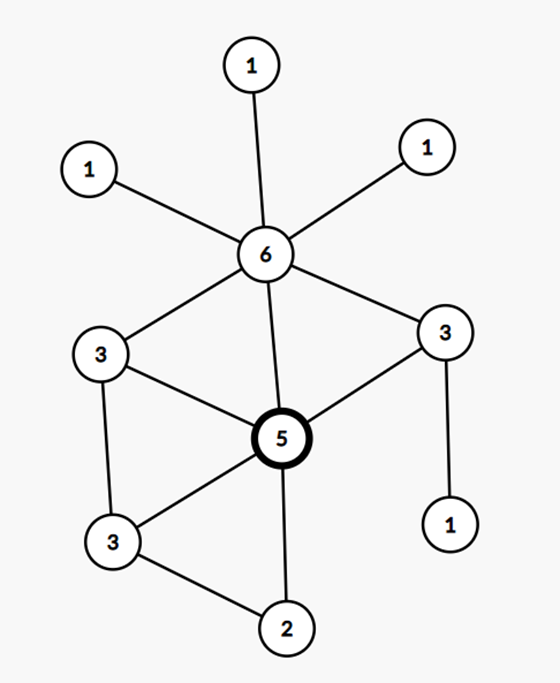
\includegraphics[scale=0.8]{graumedio.png}
    \centering
    \caption{\textbf{Exemplo de grafo não direcionado onde o número dentro de cada vértice indica seu grau.}}
    \label{fig:graumedio}
\end{figure}


\textbf{Assortatividade ($r$)}

A assortatividade traduz numericamente a preferência por vértices de uma rede para conectar a outros que são semelhantes ou diferentes em relação ao grau dos vértices em um sentido estrutural \cite{Newman_2003}.

O coeficiente de assortatividade representa o coeficiente correlação de Pearson para os pares de nós conectados. Este coeficiente, também conhecido como ``$\rho$ de Pearson'' mede o grau da correlação entre duas variáveis de escala métrica.

Os valores podem ir de $-1$ a $1$, nos quais $1$ significa uma correlação perfeita positiva entre duas variáveis, $-1$ significa uma correlação negativa perfeita e $0$ significa que uma não depende linearmente da outra, todavia, pode haver uma dependência não linear \cite{Mukaka2012}.


\textbf{Coeficiente de Agrupamento Local ($C$)}

O coeficiente de agrupamento local quantifica o quão próximo uma vizinhança de um grafo está de ser um clique, ou seja, um subgrafo completo com todas as ligações possíveis. O coeficiente de agrupamento local para um vértice é então dado pela proporção de arestas entre os vértices dentro da vizinhança dividido pelo número de arestas total que poderiam existir entre eles. O coeficiente de toda rede é a média da clusterização local \cite{Holland1971, Watts1998}. Considerando a Figura~\ref{fig:localcluster}\index{Exemplo de coeficiente de agrupamento local} e as sub figuras~\ref{fig:localcluster1}\index{Exemplo de Cluster Local 1},~\ref{fig:localcluster2}\index{Exemplo de Cluster Local 2},~\ref{fig:localcluster3}\index{Exemplo de Cluster Local 3} e~\ref{fig:localcluster4}\index{Exemplo de Cluster Local 4}, temos na primeira imagem uma rede totalmente conectada (clique). Dessa maneira, o $C = 1$, na segunda imagem, temos duas ligações realizadas de um total de três, logo, o $C = 2/3$. Na terceira, temos uma ligação existente e duas possíveis ligações adicionais, sendo assim o $C = 1/3$. No último exemplo, não temos nenhuma ligação, logo o $C = 0$.

\begin{figure}[H]
\centering
    \begin{subfigure}[b]{0.4\textwidth}
        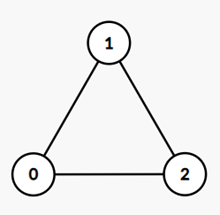
\includegraphics[width=\textwidth]{localcluster1.png}
        \centering
        \caption{\textbf{Totalmente conectada, $C = 1$.}}
        \label{fig:localcluster1}
    \end{subfigure}
    \hfill
    \begin{subfigure}[b]{0.4\textwidth}
        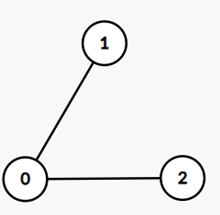
\includegraphics[width=\textwidth]{localcluster2.png}
        \centering
        \caption{\textbf{Duas ligações, o $C=2/3$.}}
        \label{fig:localcluster2}
    \end{subfigure}
    \vfill
    \begin{subfigure}[b]{0.4\textwidth}
        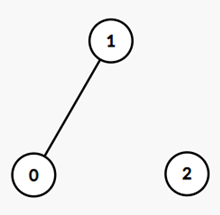
\includegraphics[width=\textwidth]{localcluster3.png}
        \centering
        \caption{\textbf{Uma ligação, $C=1/3$.}}
        \label{fig:localcluster3}
    \end{subfigure}
    \hfill
    \begin{subfigure}[b]{0.4\textwidth}
        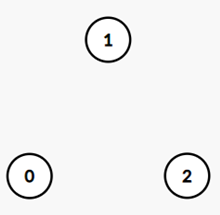
\includegraphics[width=\textwidth]{localcluster4.png}
        \centering
        \caption{\textbf{Desconectada, $C = 0$.}}
        \label{fig:localcluster4}
    \end{subfigure}
    \caption{\textbf{Exemplos de coeficiente de agrupamento local em uma rede.}}
    \label{fig:localcluster}
\end{figure}

\textbf{Transitividade (T)}

A transitividade computa a quantidade de triângulos fechados dividido pela quantidade de possíveis novos triângulos na rede. Ela considera uma tríade como um possível novo triângulo, ou seja, duas arestas com um vértice compartilhado são considerados um candidato a triângulo. Na Figura~\ref{fig:transitividade}\index{Ilustração exemplificando transitividade} mostramos uma rede na qual há dois triângulos fechados e dezesseis tríades. Sendo assim, a Transitividade dessa rede é $T = 0,375$. O cálculo poderá ser realizado utilizando a equação a seguir.

\begin{equation}
    {T}=3(\frac{\#triangulos}{\#tríades} )
\end{equation}

\begin{figure}[H]
    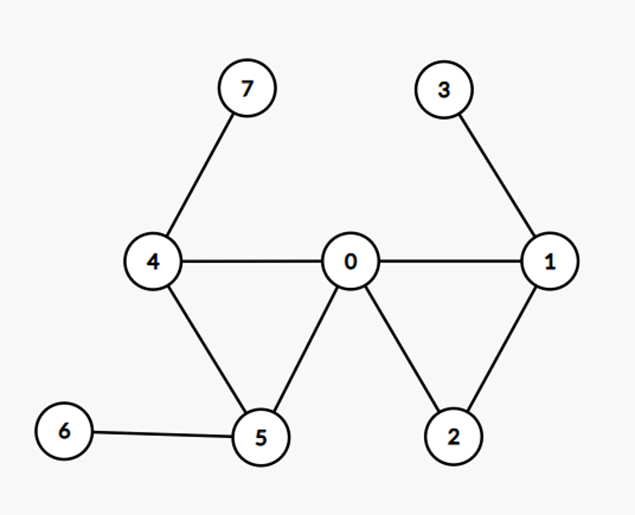
\includegraphics{transitividade.png}
    \centering
    \caption{\textbf{Exemplo de uma rede na qual temos dois triângulos fechados e dezesseis tríades, logo $T = 0,375$}}
    \label{fig:transitividade}
\end{figure}


\textbf{Comprimento Médio do Caminho Mais Curto (I)}

Mesmo os nós não estando todos diretamente ligados uns aos outros, em um componente totalmente conectado, é possível determinar um caminho para ir de um ponto ao outro. Por exemplo, se considerarmos um conjunto de nós N=[1,2,3,4,5,6], com as seguintes arestas $E = \{(0, 1),(0, 2),(0, 3),(0, 4),(0, 5),(1, 2),(4, 6) \}$, o caminho mais curto para ir do nó $2$ ao nó $6$ seria o seguinte: Nó 2 - Nó 0 - Nó 4 - Nó 6 ou $(3, 0)$ - $(0, 4)$ - $(4, 6)$. 

Para facilitar a visualização, elaboramos a Figura~\ref{fig:menorcaminho}\index{Ilustração exemplificando menor caminho}.

\begin{figure}[H]
    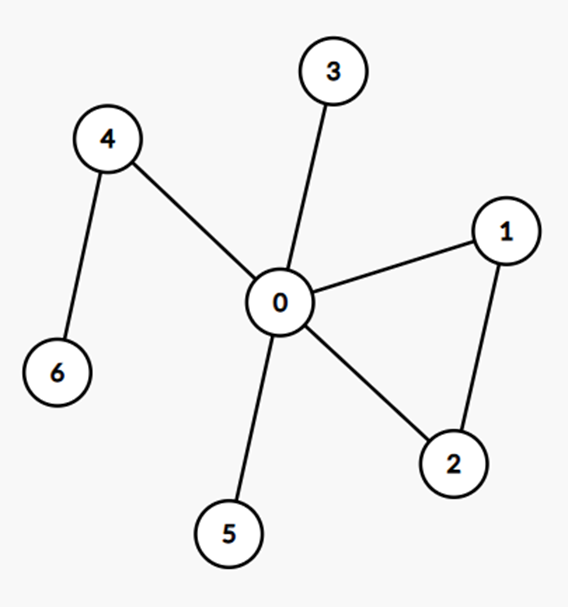
\includegraphics{menorcaminho.png}
    \centering
    \caption{\textbf{Exemplificando o menor caminho de um nó a outro.}}
    \label{fig:menorcaminho}
\end{figure}

Considerando o conceito do caminho mais curto, o comprimento médio dele seria a média aritmética para sua realização em todos os nós da rede. Ele pode ser encontrado através da seguinte fórmula:


\begin{equation}
    {I} =\sum_{v_i, v_j\in V}\frac{d(v_i, v_j)}{n(n-1)}
\end{equation}
onde $G$ é a rede, $V$ é um conjunto de nós de $G$, $d(v_i, v_j)$ é o menor caminho de nó $v_i$ para nó $v_j$ e $n$ é o número de nós na rede $G$.


\textbf{Comunicabilidade $\langle M_{v_i} \rangle$}

A comunicabilidade, diferentemente do caminho mais curto, não considera apenas os menores caminhos que conectam os nós $v_i$ e $v_j$, ela também verifica todos os possíveis caminhos que possibilitam partir de um nó e alcançar outro. Isso se deve ao fato de que em uma rede do mundo real, nem sempre o menor caminho é utilizado, diversas vezes veremos a utilização de caminhos mais longos. Além disso, os caminhos mais curtos não são muito sensíveis no que diz respeito à aparência de estruturas gargalos em uma rede, pelo contrário, o número de caminhadas é significativamente afetado pelo aparecimento dessas mudanças estruturais em uma rede \cite{Estrada2008}.

Nessa métrica, é utilizada uma fórmula para que as caminhadas mais longas tenham uma menor contribuição para a função da comunicabilidade do que as mais curtas. A comunicabilidade $M_{v_i}$ de um nó $v_i$ para todos os outros nós de uma rede é descrita por: 

\begin{equation}
%\begin{align*}
        M_{v_i}=\frac{1}{(N-1)}\sum_{j \in N}\left(\frac{1}{s!}P_{v_iv_j}+\sum_{k>s}{\frac{1}{k!}W_{v_iv_j}}\right), \: i \neq j
%\end{align*}
\end{equation}   

Na fórmula, $s$ é o tamanho do menor caminho entre $v_i$ e $v_j$, $P_{v_iv_j}$ é o número de menores caminhos entre $v_i$ e $v_j$, $W_{v_iv_j}$ é o número de caminhos conectando $v_i$ e $v_j$ de tamanho $k>s$ e $k$ é o número de passos em uma caminhada, ou seja, quantos nós ele caminha para chegar a outro ponto da rede, nos caminhos mais curtos $k$ será igual a $s$, nos demais caminhos ele será maior que $s$.

Dessa maneira, a comunicabilidade é uma métrica que analisa a rede de forma geral, computando todos os caminhos entre todos os vértices da rede. Por analisar a rede inteira, ela é bem robusta e, por utilizar todos os caminhos, a inserção ou remoção de um nó não produzirá um impacto grande na rede. E por essas suas características, escolhemos essa métrica para identificação de padrões em nosso classificador de alto nível.

É importante salientar que essa concepção possui um custo computacional elevado, e que a medida que a rede cresce, esse custo aumenta de maneira exponencial, já que a cada nova inserção, é necessário calcular para cada vértice todos os caminhos entre este e todos os outros vértices da rede.


% ---
\section{Aprendizado de Máquina e Classificação de Dados}
% ---

O conceito de classificação de dados de baixo nível em computadores acontece por meio do aprendizado de máquina tradicional. Este aprendizado pode ser descrito como sendo a capacidade de um computador ou sistema que, através de um conjunto de dados (do inglês \textit{dataset}), melhore o seu desempenho para realizar uma determinada tarefa. O sistema busca uma solução por generalização dos atributos, no qual a taxa de erros poderá servir para melhorar o próximo ciclo, buscando sempre a melhor solução para uma tarefa \cite{mitchell1997machine}.

As categorias mais clássicas para o aprendizado de máquina são:

- O aprendizado supervisionado, no qual são apresentados um grupo com etiquetas, definindo sua classe. Ele é utilizado para treinamento do algoritmo, possibilitando generalizar uma função para mapear a entrada, a saída e, posteriormente, classificar indivíduos não rotulados. Os objetivos mais comumente utilizados para esse tipo de aprendizado de máquina são classificação, regressão e redução de dimensionalidade.

- O aprendizado por reforço, um tipo de aprendizado no qual pode-se definir um objetivo (\textit{target}) e, quando o algoritmo retorna resultados condizentes a esse objetivo, ele recebe uma espécie de recompensa. Da mesma forma, quando ele vai de maneira oposta ao objetivo, ele recebe uma penalização, sendo que essa resposta recebe o nome de \textit{feedback}. O algoritmo, então, tende a corrigir seu comportamento e montar um modelo. Esse algoritmo pode ser utilizado para máquina aprender a jogar, ou para projetar uma determinada peça aerodinâmica, por exemplo.

- O aprendizado não supervisionado, no qual não são passados rótulos no grupo de dados. O algoritmo tenta de maneira autônoma identificar qualquer similaridade e, dessa maneira, forma grupos que podem ou não fazer sentido para a solução do problema desejado. Esse tipo de algoritmo normalmente é utilizado para formação de \textit{clusters} ou grupos, podendo ainda ser utilizados em outras aplicações.

É possível também fazer uso conjunto de diferentes categorias de algoritmos, para obtenção de outros resultados, como, por exemplo, criar um classificador com uma espécie de aprendizado profundo (\textit{deep learning}) utilizando a saída de um algoritmo de não supervisionado como a entrada de um algoritmo supervisionado com objetivo de classificação.

Para o presente trabalho, como nosso objetivo é classificar um conjunto de exemplos, focaremos na primeira categoria.

Os algoritmos de aprendizado de máquina podem ainda ser categorizados por sua saída, sendo estas as mais comuns:

Classificação: Utilizada quando possuímos duas ou mais classes e desejamos que o conjunto de entrada seja distribuído entre elas, normalmente se trata de um aprendizado supervisionado.

Regressão: a regressão é bem semelhante à classificação, mas ela possui saídas contínuas, diferentemente da classificação na qual as saídas são discretas.

Em aprendizado supervisionado, o qual utilizamos para classificação, temos um conjunto de dados com seus devidos rótulos de classificação (conjunto de treinamento). Através de um conjunto de treinamento, será treinado um classificador, o qual poderá predizer a classe de um novo exemplo não rotulado.

Considerando um conjunto de dados de treinamento: $(X, Y) = {(x_1, y_1), ...,(x_n, y_n)}$, onde $x_i$ é um item de dado e $y_i$ é o correspondente rótulo de classe, o objetivo do treinamento é encontrar uma função para aproximar os pares, tal que $y_i \approx f(x_i)$. Após o processo de treinamento, o algoritmo será capaz predizer e classificar corretamente novos exemplos do mesmo problema, utilizando o classificador $f$ encontrado na fase de treinamento.

Devido à importância deste paradigma de aprendizado em várias aplicações reais, muitas técnicas de classificação foram desenvolvidas \cite{Alpaydin2009, Goodfellow2016, Haykin1998, Vapnik2008}, tais como o K-vizinhos mais próximos (KNN), Análise Linear Discriminante (LDA), Naive-Bayes, redes neurais, aprendizado profundo, Support Vector Machines (SVM), Árvore de Decisão entre outras.

Essencialmente, as técnicas tradicionais de classificação de dados realizam treinamento e classificação utilizando atributos físicos dos dados (por exemplo, distância, similaridade ou distribuição), as quais são chamadas de técnicas de \textit{classificação de baixo nível}. Frequentemente, os itens de dados não são pontos isolados no espaço de atributos, mas tendem a formar certos padrões. A classificação de dados que considera a formação de padrões dos dados de entrada, além dos atributos físicos, é referida como\textit{ classificação de alto nível}.
Embora cada uma delas possua suas próprias características, as técnicas tradicionais de classificação normalmente compartilham a mesma heurística: basicamente, o processo de classificação consiste em dividir o espaço de dados em subespaços, cada um representando uma classe. O classificador treinado serve para definir as fronteiras de decisão no espaço de dados e a indução de rótulo verifica a posição relativa de cada instância sem rótulo em relação às fronteiras. Estes subespaços não são sobrepostos no caso de classificação \textit{crisp}, mas podem ser ligeiramente sobrepostos, no caso de classificação \textit{fuzzy}. De qualquer forma, distorções fortes nas formas das classes ou subespaços sobrepostos não são permitidos em geral. Em outras palavras, técnicas de classificação de dados tradicionais funcionam de acordo com as características físicas (similaridade, distância, ou distribuição) dos dados de treinamento, ignorando muitas outras relações intrínsecas e semânticas entre os itens de dados, que normalmente geram classes em formas complexas no espaço de dados. Por outro lado, é sabido que o cérebro (animal) humano pode identificar padrões de acordo com o significado semântico dos dados de entrada. Por isso, é interessante realizar a classificação, além do conceito geralmente aplicado de divisão do espaço de dados. Neste contexto, técnicas baseadas em rede podem fazer contribuições para a realização de classificação de dados a partir de pontos de vista bastante diferentes em vez da forma de divisão do espaço de dados.
 
Dessa maneira, os classificadores de baixo nível (tradicionais) podem classificar de maneira equivocada alguns problemas nos quais um humano conseguiria ver claramente um padrão.

A Figura~\ref{fig:padraovisual}\index{Ilustração de problema onde existe um padrão e os dados desse padrão se sobrepõe aos dados de outras classes} ilustra muito bem um exemplo dessa situação, considerando em um plano, onde os círculos representam a classe A e o os quadrados representam a classe B, os círculos em azul claro tendem a ser classificados corretamente por um algoritmo de baixo nível, bem como os quadrados em vermelho claro, porém, os círculos em azul escuro tendem a gerar uma confusão nesse tipo de algoritmo, já que levando em conta características físicas ou de distribuição eles provavelmente serão classificados como classe B. Um humano observando a imagem, facilmente identificaria o padrão e, provavelmente, classificaria corretamente. Essa é então a principal diferença de se utilizar um classificador de baixo nível ou um classificador de alto nível, alguns problemas necessitam que padrões de formação de dados sobrepostos sejam analisados, não apenas medidas ou características físicas.

\begin{figure}[H]
    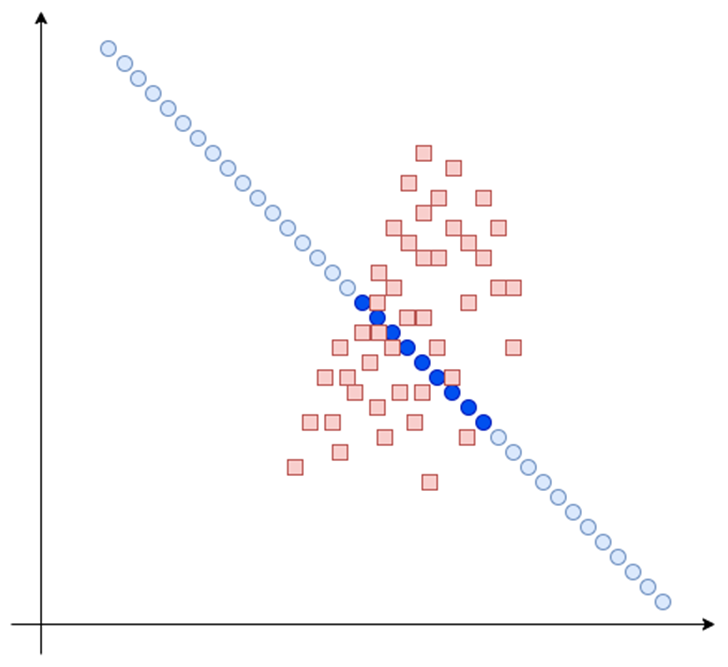
\includegraphics[width=\textwidth]{padraovisual.png}
    \centering
    \caption{\textbf{Exemplo de problema no qual dados possuem um padrão visual de formação de dados e tais dados estão sobrepostos a dados de outras classes.}}
    \label{fig:padraovisual}
\end{figure}

\section{Classificação de Dados de Alto Nível}

A classificação de alto nível procura encontrar não somente características físicas e de distribuição, mas também o padrão de formação dos dados. Esse tipo de identificação permite que exemplos sobrepostos ou próximos em um plano cartesiano sejam classificados em suas respectivas classes. O classificador de alto nível utiliza medidas de rede para conseguir capturar os padrões da rede \cite{silva2012a, Colliri2018, cupertino2017, CARNEIRO2019}.

A ideia original de construir uma técnica híbrida de classificação de baixo e alto níveis foi proposta em \cite{silva2012a, silva2015} e estendida em \cite{carneirozhao2018, Colliri2018, carneiro2014, carneiro2016, covoes2017, cupertino2017, CARNEIRO2019}. No esquema original, a classificação de baixo nível pode ser implementada por qualquer técnica de classificação tradicional, enquanto que a técnica de alto nível explora as propriedades topológicas complexas da rede construída a partir dos dados de entrada. No trabalho introduzido em \cite{silva2012a}, a classificação de alto nível é realizada usando-se três medidas de rede: assortatividade, coeficiente de agrupamento e grau médio. Já em \cite{silva2015}, a medida do comprimento transiente e ciclo de caminhada de turista foi utilizada para classificação. Em ambos os casos, a classificação é realizada pela verificação de conformidade do padrão formado de cada rede (cada classe) para cada dado de teste i.e., um item de teste é atribuído para aquela classe onde sua inserção na correspondente rede causou a menor variação nas medidas em consideração. Em \cite{carneirozhao2018, Colliri2018, cupertino2017}, a parte de classificação de baixo nível foi eliminada e técnicas puras de classificação de alto nível foram propostas. Em \cite{Colliri2018} são empregadas várias medidas de rede (Grau médio, Assortatividade, Coeficiente de Agrupamento Local, Transitividade, Comprimento Médio do Caminho mais Curto), que introduzem um conjunto de parâmetros representativos do peso de cada medida e que incrementam uma dificuldade considerável para serem definidos. Em \cite{carneirozhao2018} foi utilizada uma única métrica,  uma implementação derivada da métrica \textit{pagerank} e ela foi capaz de encontrar características suficientes para resolução do problema. Em \cite{cupertino2017} foi utilizada a métrica \textit{random walk} e esta conseguiu capturar informações físicas e estruturais dos dados, permitindo uma correta classificação. Em nosso trabalho utilizaremos apenas uma métrica, a comunicabilidade \cite{Estrada2008}. Por se tratar de uma métrica que analisa dados de toda a rede, medindo não somente as menores distâncias, mas sim, todas as distâncias entre todos os vértices da rede, por isso, acreditamos que ela seja capaz de capturar padrões de formação dos dados, levando em consideração características físicas e estruturais. Sendo assim, introduzimos uma técnica de classificação de alto nível modificada usando essa medida de rede.

A classificação alto nível é composta por duas etapas, a fase de treinamento e a fase de classificação. 

Durante a fase de treinamento, utilizamos o conjunto de treinamento para montagem das redes. Para cada classe existente será montado uma rede. Uma medida ou um conjunto de medidas é calculado para a rede de cada classe para representar o padrão formado da rede.

Na fase de classificação, calculamos o impacto que a inserção de um item provocaria em cada uma das redes. Esse impacto é comparado à matriz de impacto da rede onde ele tentou ser inserido. Sempre que houver uma grande variação nas medidas de uma rede, demonstra que aquele item não está em conformidade com a rede na qual ele tentou ser inserido. Da mesma maneira, acontecendo o inverso, ou seja, caso a variação de medidas for pequena e estiver em conformidade com o impacto de inserções na mesma rede, demonstram por sua vez que existe semelhança com o padrão aprendido para aquela rede, determinando que essa rede será a melhor escolha para a predição.

Essa característica permite que encontremos padrões entre os itens e não somente medidas e aspectos físicos, possibilitando que a máquina encontre padrões nos dados e que classificadores de baixo nível teriam dificuldade de encontrar e consequentemente de classificar.

Pesquisas comprovaram que um algoritmo híbrido que faz uso de redes complexas e medidas de rede para encontrar padrões foi capaz de resolver problemas de conjunto de dados sintéticos e reais com índice maior de acurácia do que classificadores de baixo nível. Também foi capaz de identificar letras manuscritas com uma margem grande de acurácia, comparado a outros algoritmos tradicionais \cite{silva2012a}.

Outros estudos demonstraram ainda que um classificador de alto nível puro obteve também resultados superiores aos de algoritmos tradicionais para classificar conjunto de dados com padrões definidos, sejam eles conjunto de dados artificiais, como por exemplo \textit{Blobs}, \textit{Circles}, \textit{Moons}, bem como para conjunto de dados reais, como por exemplo \textit{Breast} câncer, \textit{Digits}, \textit{Iris}, \textit{Zoo} \cite{Colliri2018}.


\chapter{Materiais e Métodos}
Neste capítulo serão apresentados o conjunto de dados utilizado neste trabalho e o método proposto de classificação de imagens raio-X de tórax de pacientes com COVID-19, Pneumonia e saudáveis.

\section{Conjunto de Dados}
Para realizarmos nossa análise, montamos um conjunto de dados a partir da junção de quatro conjuntos abertos na internet. O primeiro foi obtido a partir do repositório \textit{GitHub} do Dr. Joseph Paul Cohen \cite{repo1}, o segundo foi obtido do repositório \textit{github} da Dra Audrey Gina Chung \cite{repo2}, o terceiro é um repositório da Actualmed, que foi compilado pelos doutores José Antonio Heredia Álvaro e Pau Agustí Ballester da Universitat Jaume I \cite{repo3} e o último é um conjunto de imagens da Sociedade de Radiologia dos Estados Unidos (RSNA) e foi divulgado durante uma competição que desafiava o desenvolvimentos dos melhores algoritmos para identificação de sinais de pneumonia \cite{repo4}.

Nosso conjunto de imagens gerado a partir dessa junção totalizou 13861 imagens, das quais 436 imagens são de pacientes acometidos com COVID-19, outras 5359 imagens são de pacientes com pneumonia e as últimas 7966 imagens restantes foram capturadas de pacientes saudáveis.

Posteriormente, para um segundo teste, utilizamos um outro conjunto de dados obtidos através do repositório tawsifurrahman \cite{repo5}. Desse repositório, utilizamos apenas as imagens de COVID-19. No momento da consulta, ele possuía 219 imagens para esse tipo de paciente.

As imagens possuem dimensões diferentes. Para podemos utilizar em nosso classificador, recortamos as imagens maiores padronizando o tamanho, esse processo seguiu o seguinte conceito: Obtemos as dimensões da menor imagem do conjunto de dados e nas imagens maiores medimos o ponto central da imagem e, a partir dele, extraímos o conteúdo, ou seja, retiramos do centro da imagem um retângulo com as dimensões da menor imagem.

As Figuras~\ref{fig:covid1}\index{Exemplo 1 de Raio x de paciente com COVID-19} e~\ref{fig:covid2}\index{Exemplo 2 de Raio x de paciente com COVID-19} são exemplos de imagens do nosso conjunto de dados de pacientes com corona vírus, as Figuras~\ref{fig:pneumo1}\index{Exemplo 1 de Raio x de paciente com Pneumonia} e~\ref{fig:pneumo2}\index{Exemplo 2 de Raio x de paciente com Pneumonia} mostram pacientes com pneumonia e, por último, as Figuras~\ref{fig:saudavel1}\index{Exemplo 1 de Raio x de paciente saudável} e~\ref{fig:saudavel2}\index{Exemplo 2 de Raio x de paciente saudável} são imagens de pessoas saudáveis.

\begin{figure}[H]
    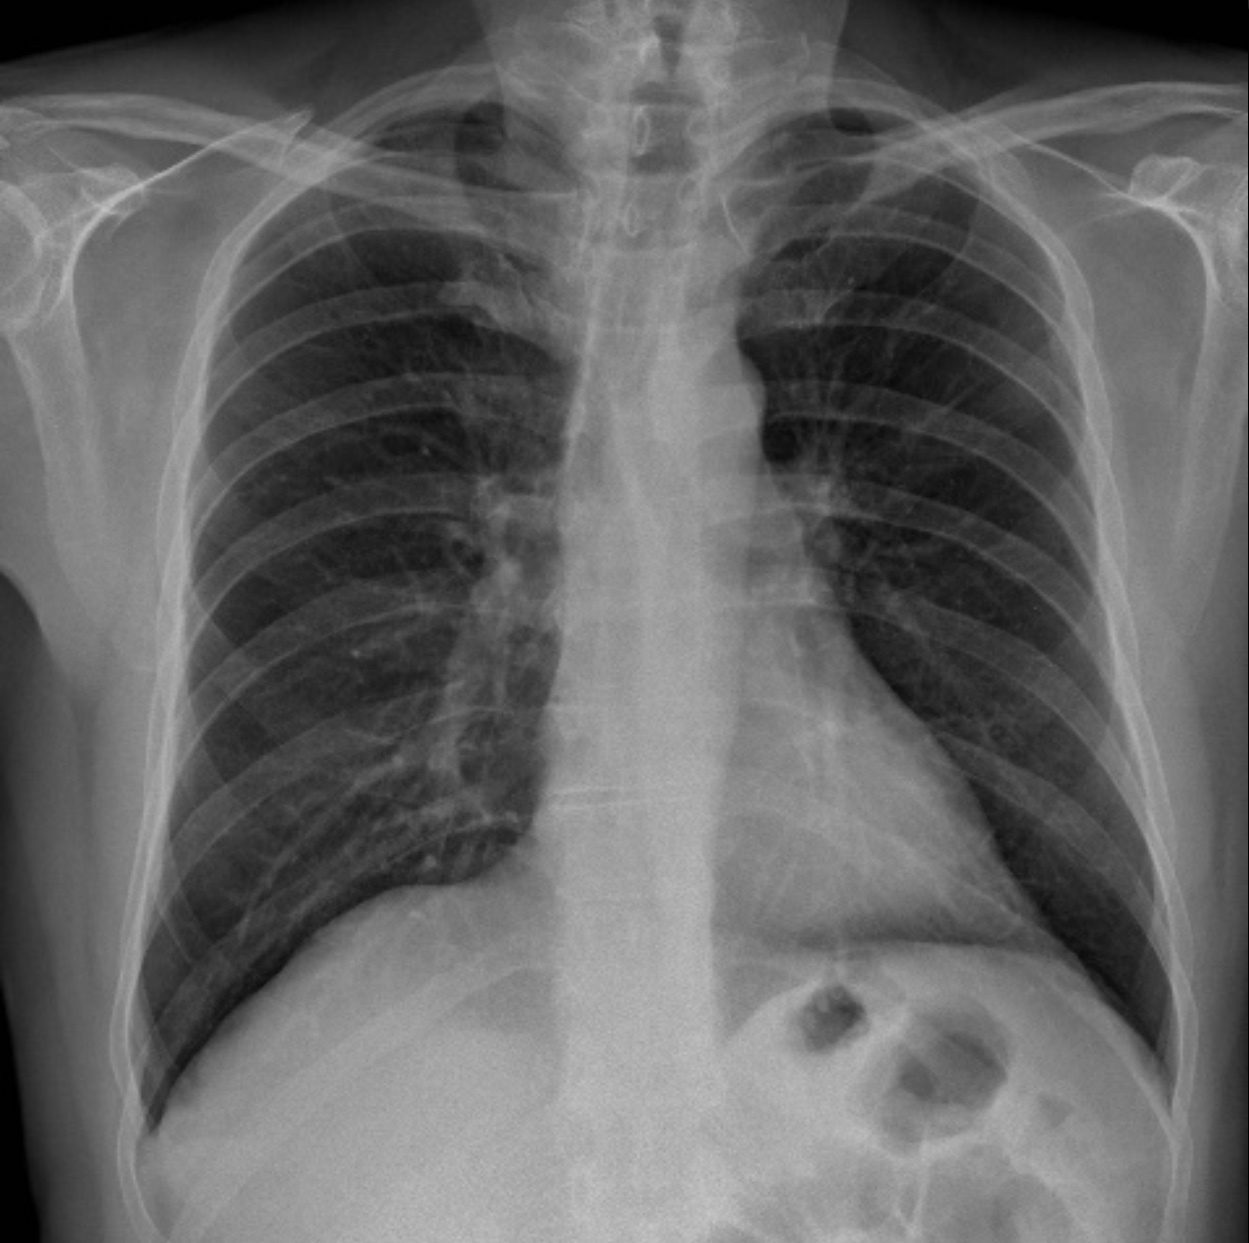
\includegraphics[scale=0.22]{covid1.jpeg}
    \centering
    \caption{\textbf{Exemplo de radiografia de paciente com COVID-19 \cite{repo1}.}}
    \label{fig:covid1}
\end{figure}

\begin{figure}[H]
    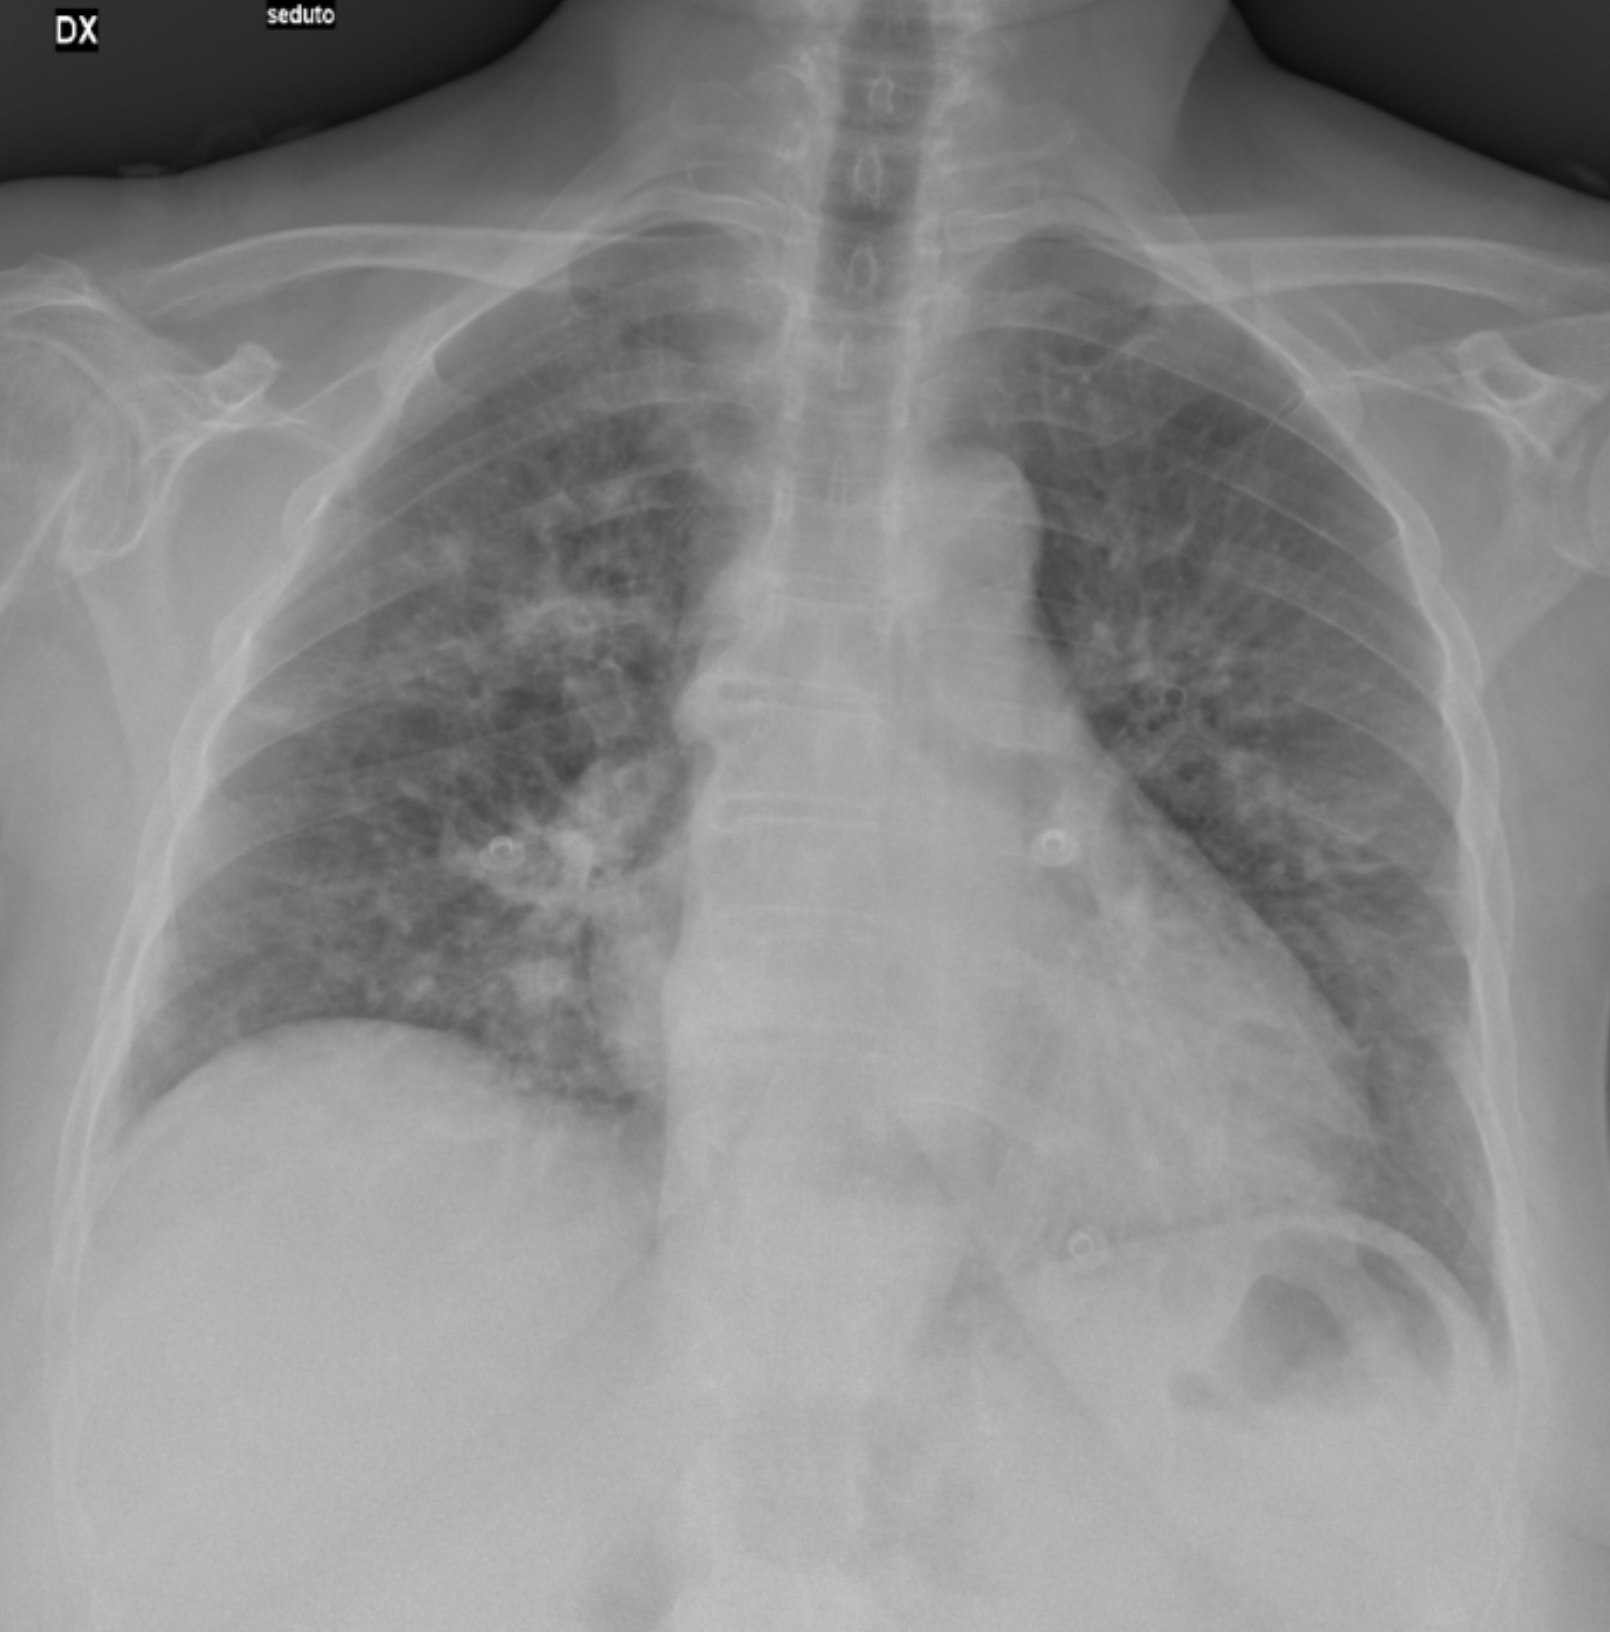
\includegraphics[scale=0.18]{covid2.jpeg}
    \centering
    \caption{\textbf{Exemplo de radiografia de paciente com COVID-19 \cite{repo1}.}}
    \label{fig:covid2}
\end{figure}

\begin{figure}[H]
    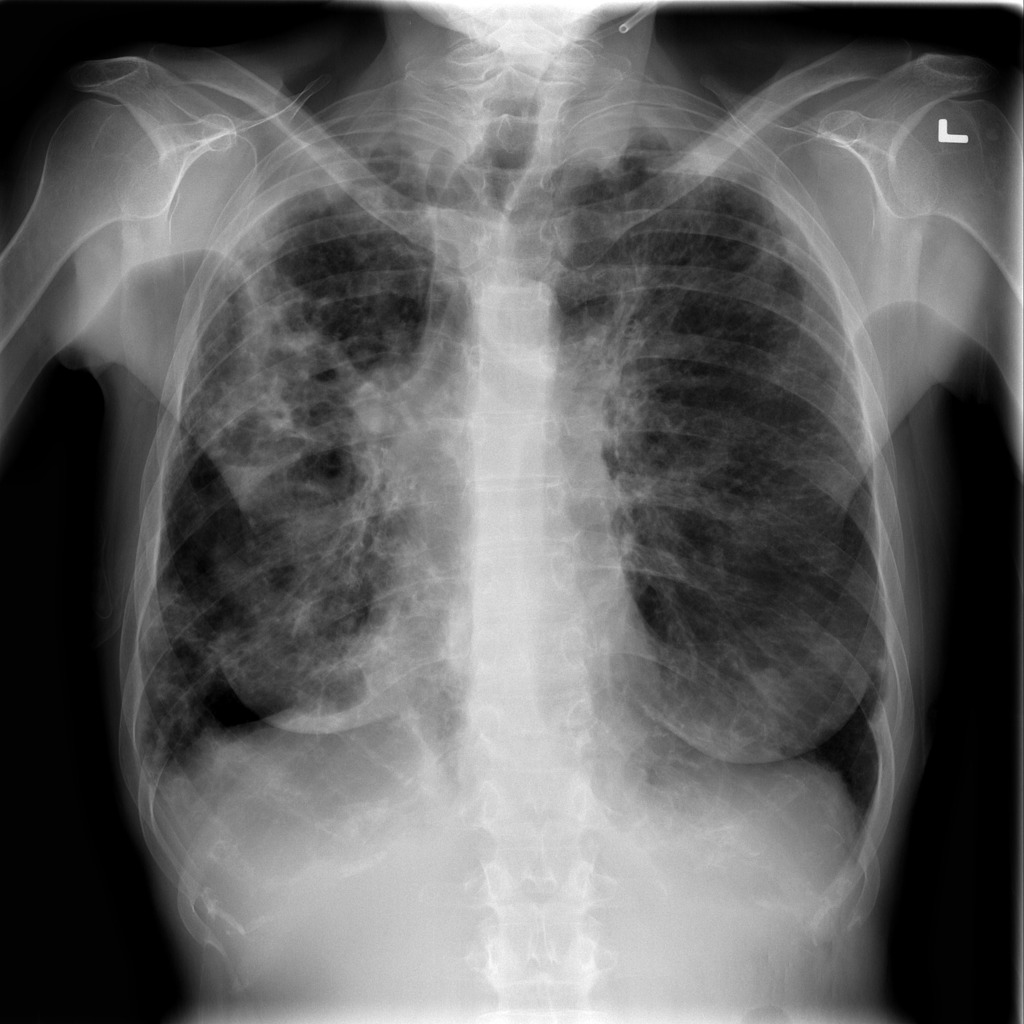
\includegraphics[scale=0.28]{pneumo1.png}
    \centering
    \caption{\textbf{Exemplo de radiografia de paciente com Pneumonia \cite{repo4}.}}
    \label{fig:pneumo1}
\end{figure}

\begin{figure}[H]
    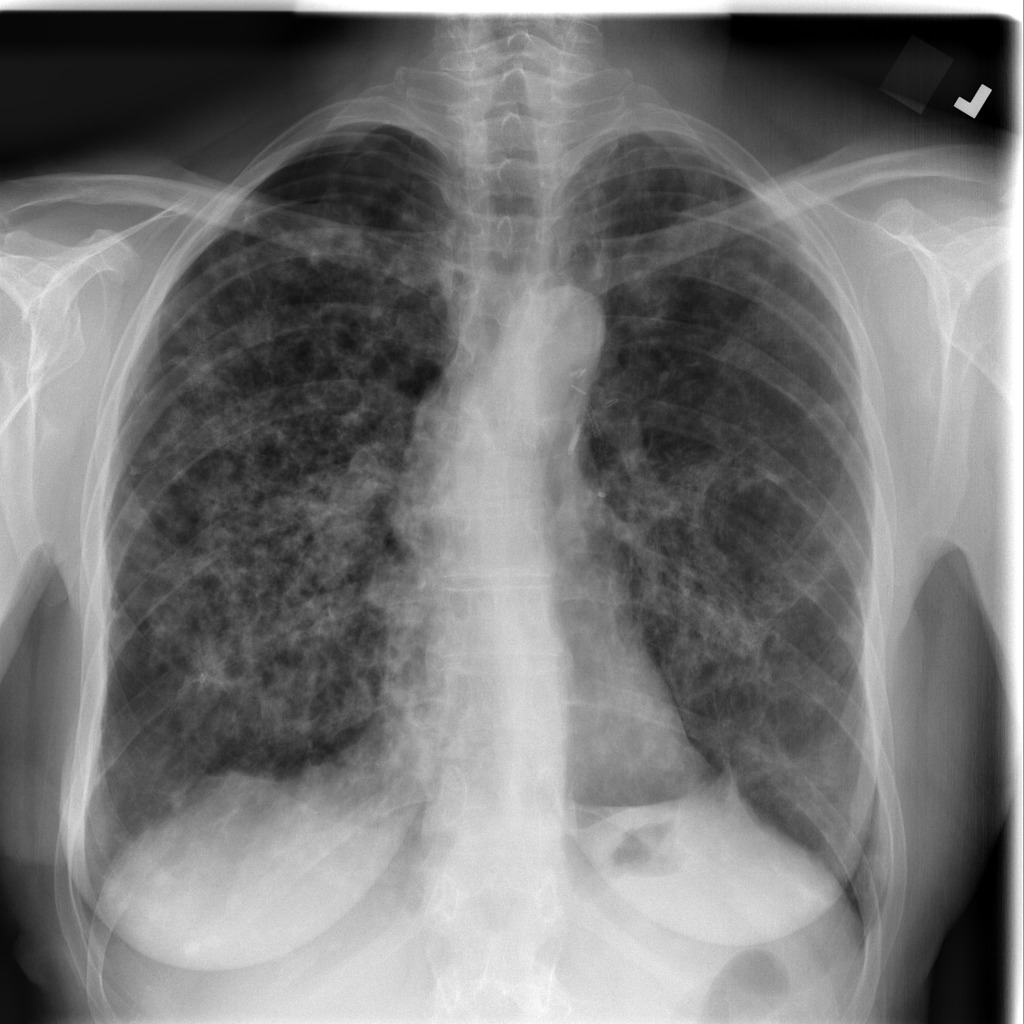
\includegraphics[scale=0.28]{pneumo2.png}
    \centering
    \caption{\textbf{Exemplo de radiografia de paciente com Pneumonia \cite{repo4}.}}
    \label{fig:pneumo2}
\end{figure}

\begin{figure}[H]
    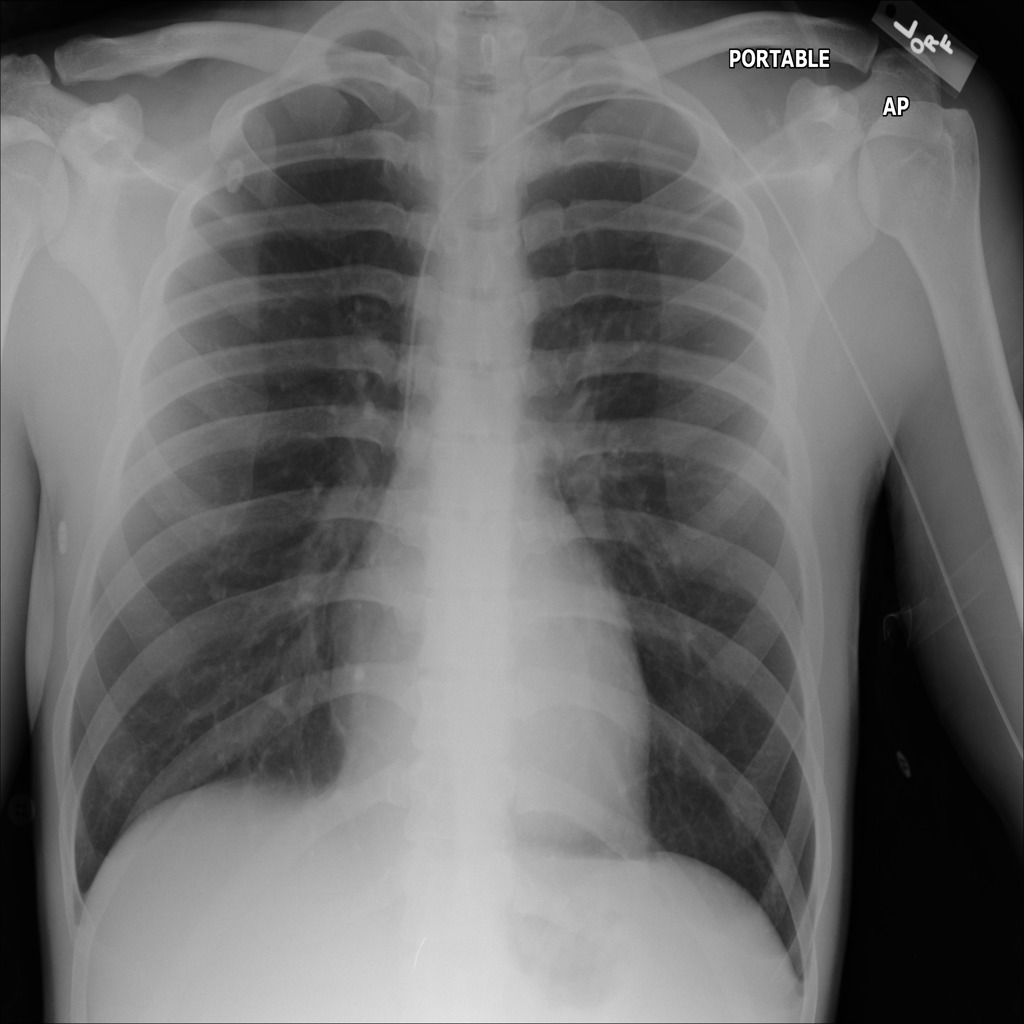
\includegraphics[scale=0.3]{saudavel1.png}
    \centering
    \caption{\textbf{Exemplo de radiografia de paciente com saudável \cite{repo4}.}}
    \label{fig:saudavel1}
\end{figure}

\begin{figure}[H]
    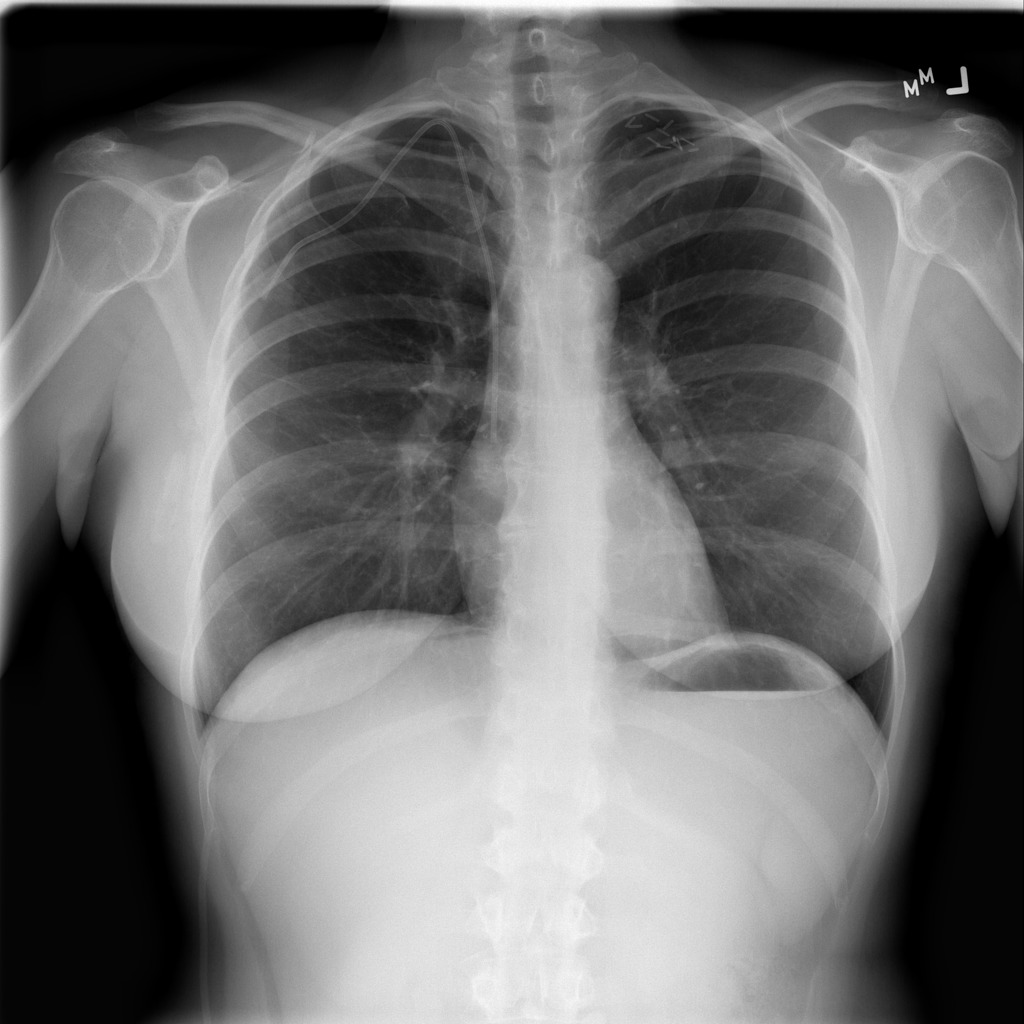
\includegraphics[scale=0.3]{saudavel2.png}
    \centering
    \caption{\textbf{Exemplo de radiografia de paciente com saudável \cite{repo4}.}}
    \label{fig:saudavel2}
\end{figure}

Nas imagens dos quadros da Figura~\ref{fig:quadroimagens}\index{Imagens de Raio-X de pacientes com COVID-19, pneumonia e saudáveis}, podemos observar que cada classe apresenta um padrão definido. Os pulmões saudáveis mostram alta transparência e alta visibilidade de costelas. Por outro lado, os pulmões de pacientes com COVID-19 apresentam baixa transparência e muitas fibras irregulares \cite{guan2020}. As imagens de pacientes de pneumonia mostram situações intermediárias \cite{ARAUJO-FILHO2020}.

\begin{figure}[H]
\centering
    \begin{subfigure}[b]{0.49\textwidth}
        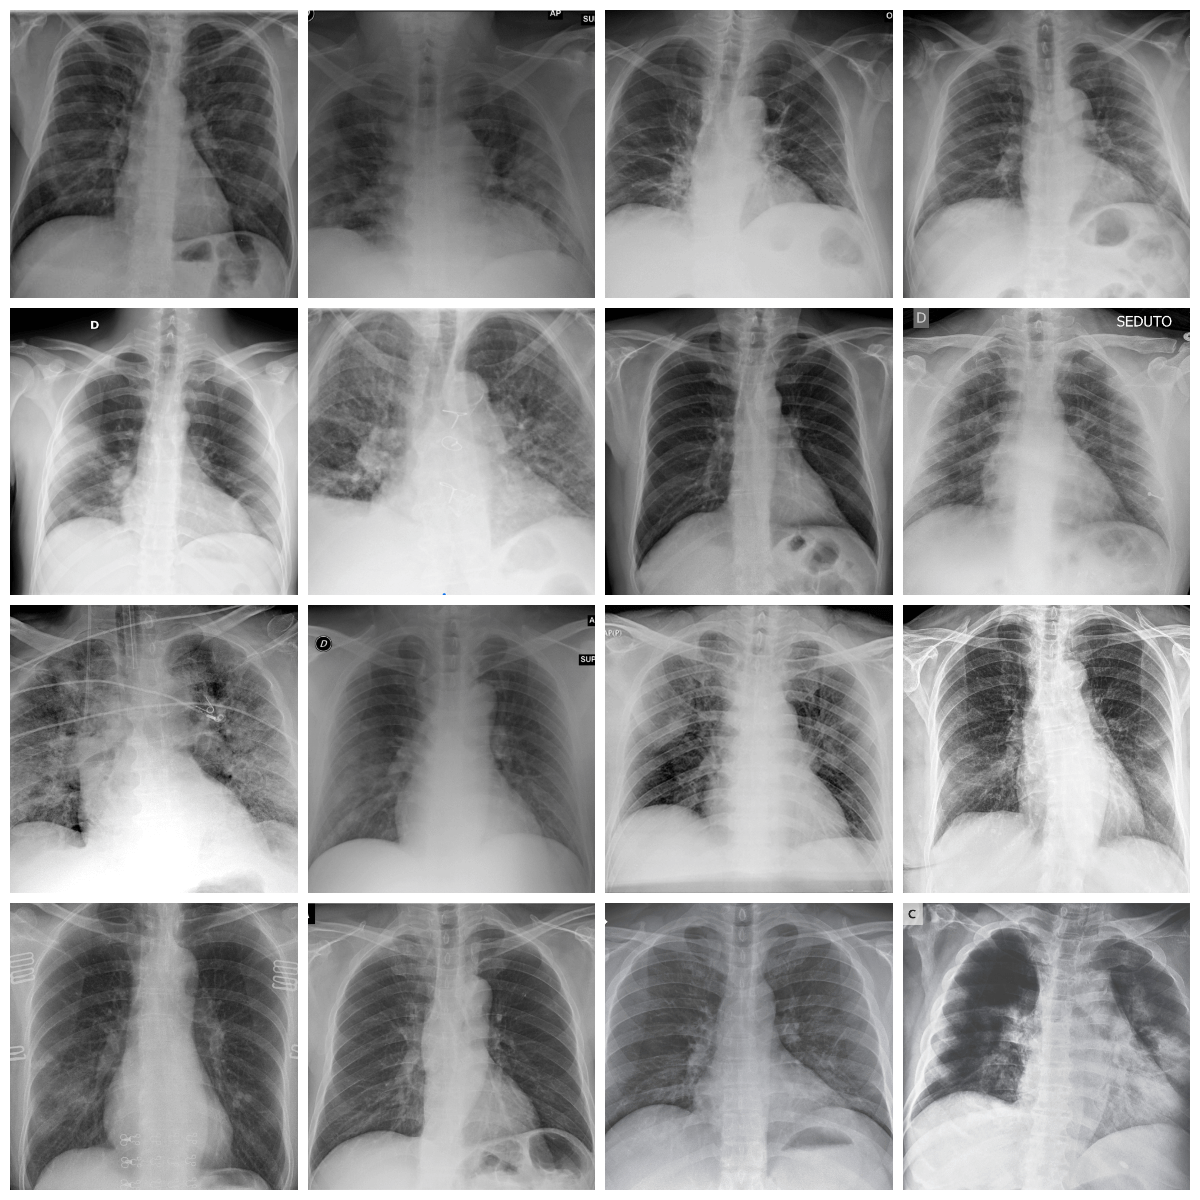
\includegraphics[width=\textwidth]{quadrocovid.png}
        \centering
        \caption{\textbf{Raio-X de pessoas com COVID-19.}}
        \label{fig:quadrocovid}
    \end{subfigure}
    \hfill
    \begin{subfigure}[b]{0.49\textwidth}
        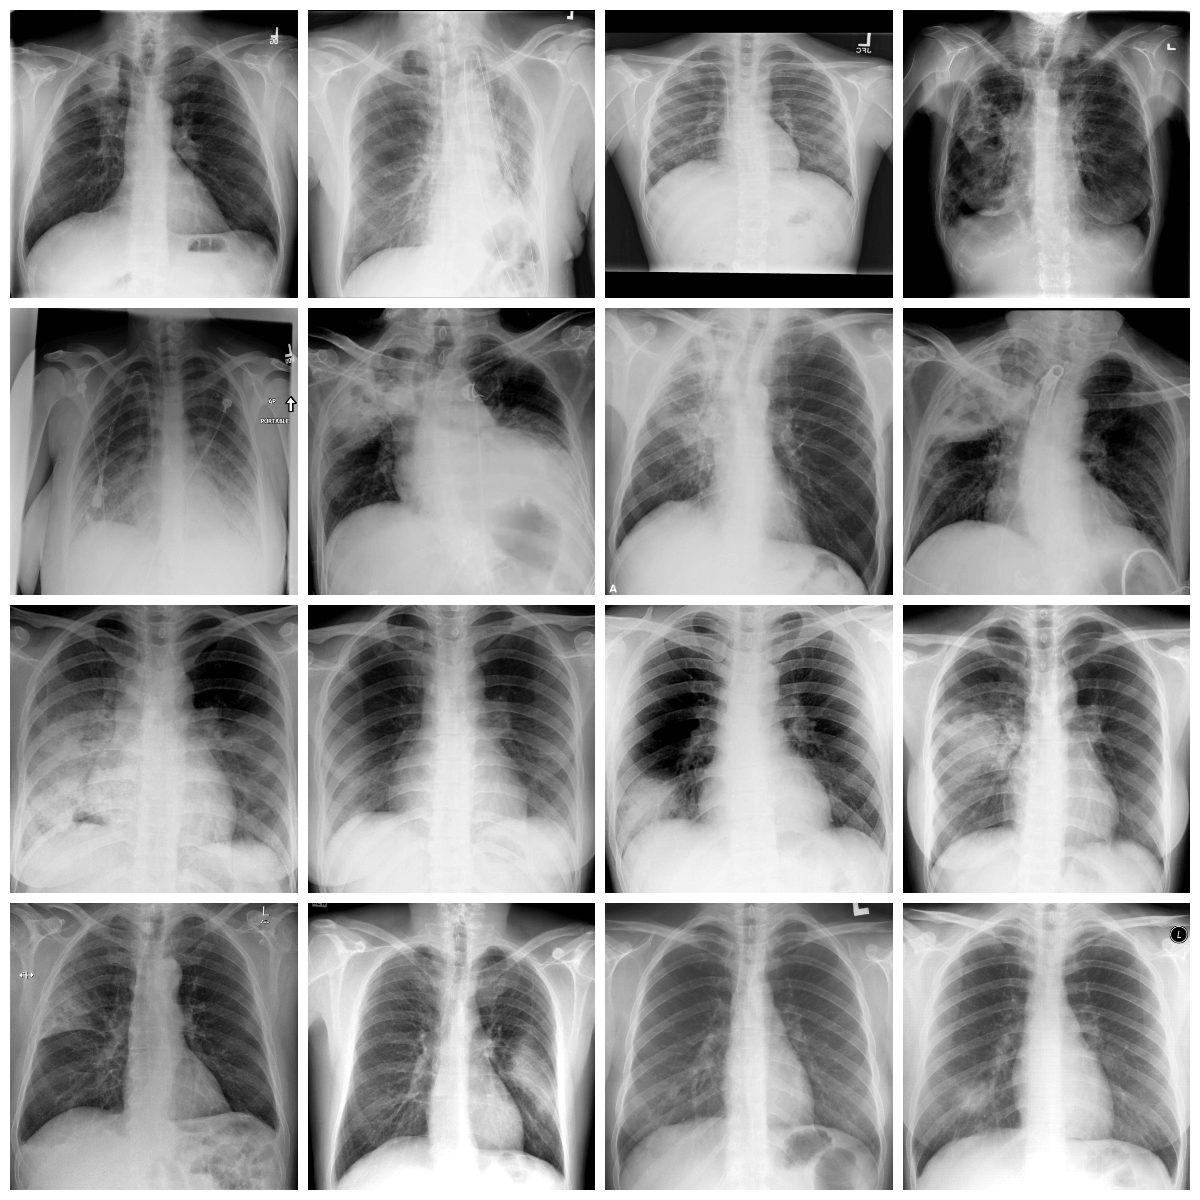
\includegraphics[width=\textwidth]{quadropneumo.png}
        \centering
        \caption{\textbf{Raio-X de pessoas com pneumonia.}}
        \label{fig:quadropneumo}
    \end{subfigure}
    \vfill
    \begin{subfigure}[b]{0.49\textwidth}
        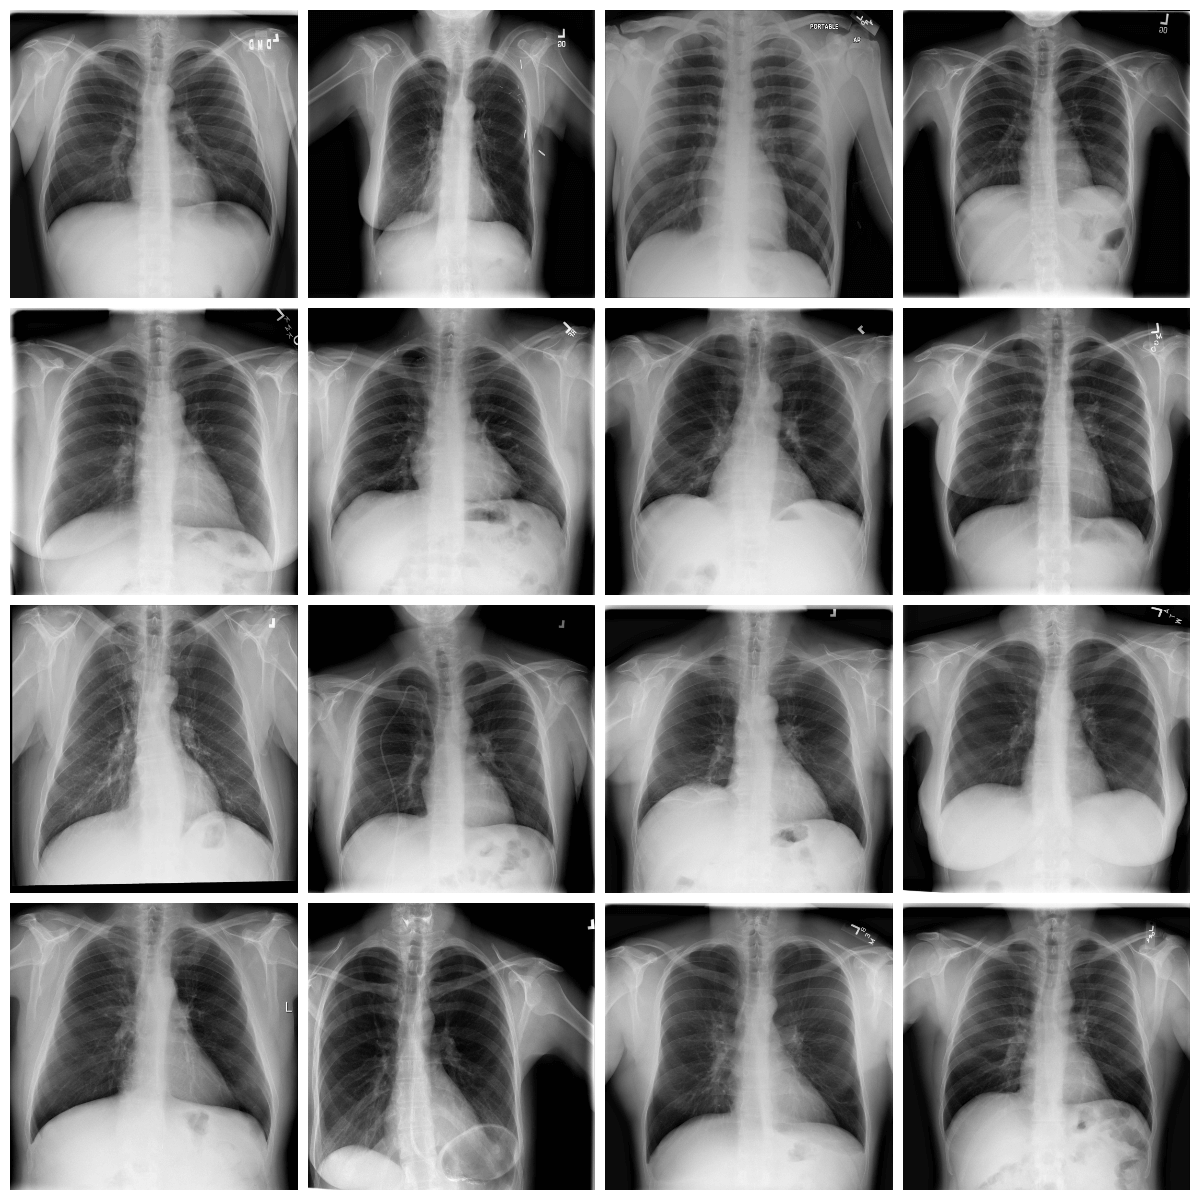
\includegraphics[width=\textwidth]{quadrosaudavel.png}
        \centering
        \caption{\textbf{Raio-X de pessoas saudáveis.}}
        \label{fig:quadrosaudavel}
    \end{subfigure}
    \caption{\textbf{Exemplos imagens do conjunto de dados.}}
    \label{fig:quadroimagens}
\end{figure}

%\pagebreak
\section{Método Proposto}
Nesta seção, será apresentado o método proposto de classificação de imagens de tórax passo a passo.

\subsection{Pré-Processamento de Imagens}
Inicialmente, utilizamos uma transformação morfológica em todas as imagens em uma etapa que denominamos de fase de pré-processamento, na qual aplicamos a transformação de abertura imagem a imagem. Essa técnica consiste em aplicar a transformação morfológica erosão seguida da transformação morfológica dilatação. O pré-processamento tem como objetivo redução de ruídos de imagens originais \cite{haralick1992,vernon1991}.

Especificamente, a função erosão corrói a imagem usando um elemento de estruturação especificado que determina a forma de uma vizinhança de pixel sobre a qual o mínimo é obtido \cite{gonzalez1992,haralick1992}, seguindo a fórmula a seguir:

\begin{center}
\scalebox{1.5}{
$dst(x,y)= \min_{(x',y'): element(x',y')\neq0}src(x+x',y+y')$
}
\end{center}

A Figura~\ref{fig:imagemoriginal}\index{Imagem original para exemplo de transformação morfológica} exemplifica a imagem original, sem nenhuma transformação aplicada. A Figura~\ref{fig:erosao}\index{Imagem após transformação de erosão} demonstra a aplicação da transformada morfológica erosão, na qual podemos ver o “desgaste” dos pixels reduzindo o diâmetro do texto.

A função dilatação dilata a imagem de origem usando um elemento de estruturação especificado que determina a forma de uma vizinhança de pixel sobre a qual o máximo é obtido \cite{gonzalez1992,haralick1992}, seguindo a fórmula a seguir:

\begin{center}
\scalebox{1.5}{
$dst(x,y)= \max_{(x',y'): element(x',y')\neq0}src(x+x',y+y')$
}
\end{center}

A Figura~\ref{fig:dilatacao}\index{Imagem após transformação de dilatação} é o resultado da Figura~\ref{fig:imagemoriginal}\index{Imagem original para exemplo de transformação morfológica} após execução da transformada morfológica de dilatação. É possível ver que o texto ficou dilatado. \cite{gonzalez1992,haralick1992}

A aplicação dessas duas transformações na sequência reduz ruídos em imagens produzidas por equipamentos de raio-x com qualidade inferior. A Figura~\ref{fig:imagemruido}\index{Imagem com ruído para exemplificar técnica de abertura} representa uma imagem com um ruído no plano de fundo. Esse ruído pode ser atenuado aplicando a transformação de abertura. A Figura~\ref{fig:opening}\index{Imagem com ruído após aplicarmos técnica de abertura} é o resultado da aplicação dessa transformada na Figura~\ref{fig:imagemruido}\index{Imagem com ruído para exemplificar técnica de abertura}, sendo possível observar que foi preservado o conteúdo que desejávamos manter e o ruído foi reduzido. É importante ressaltar que um ruído natural por não possuir muitas vezes padrão, pode ser mais difícil de ser removido, dessa maneira, foi necessária uma análise para definir os melhores parâmetros para utilização da transformada.

\begin{figure}[H]
    
\includegraphics{imagemoriginal.png}
    \centering
    \caption{\textbf{Imagem original.}}
    \label{fig:imagemoriginal}
\end{figure}

\begin{figure}[H]
    
\includegraphics[scale=0.6]{erosao.png}
    \centering
    \caption{\textbf{Imagem resultante da transformada de erosão.}}
    \label{fig:erosao}
\end{figure}

\begin{figure}[H]
    
\includegraphics[scale=0.6]{dilatacao.png}
    \centering
    \caption{\textbf{Imagem resultante da transformada de dilatação.}}
    \label{fig:dilatacao}
\end{figure}

\begin{figure}[H]
    
\includegraphics{imagemruido.png}
    \centering
    \caption{\textbf{Imagem original com ruído artificial.}}
    \label{fig:imagemruido}
\end{figure}

\begin{figure}[H]
    
\includegraphics[scale=0.6]{opening.png}
    \centering
    \caption{\textbf{Imagem resultante da transformada de abertura na imagem com ruído.}}
    \label{fig:opening}
\end{figure}

Considerando, agora o cenário real de nosso problema, as Figuras~\ref{fig:covidopening}\index{Imagem resultante da transformada de abertura na Figura~\ref{fig:covid1}},~\ref{fig:pneumoopening}\index{Imagem resultante da transformada de abertura na Figura~\ref{fig:pneumo1}} e~\ref{fig:saudavel2opening}\index{Imagem resultante da transformada de abertura na Figura~\ref{fig:saudavel2}} ilustram o resultado da aplicação dessa transformada nas figuras. Podemos visualizar que além do tratamento da imagem, a transformada removeu ainda parte do texto na Figura~\ref{fig:saudavel2opening}\index{Imagem resultante da transformada de abertura na Figura~\ref{fig:saudavel2}}, o que é ideal para garantir que nosso classificador não utilize uma anotação como parâmetro para identificação de padrão. É possível definir também a intensidade de aplicação dessa técnica. Após testarmos diferentes parâmetros utilizamos um \textit{kernel} de 12 por 12 preenchidos com um. A utilização dessa transformada incrementou em aproximadamente 5\% a acurácia de nosso classificador de alto nível.

\begin{figure}[H]
\centering
    \begin{subfigure}[b]{0.45\textwidth}
        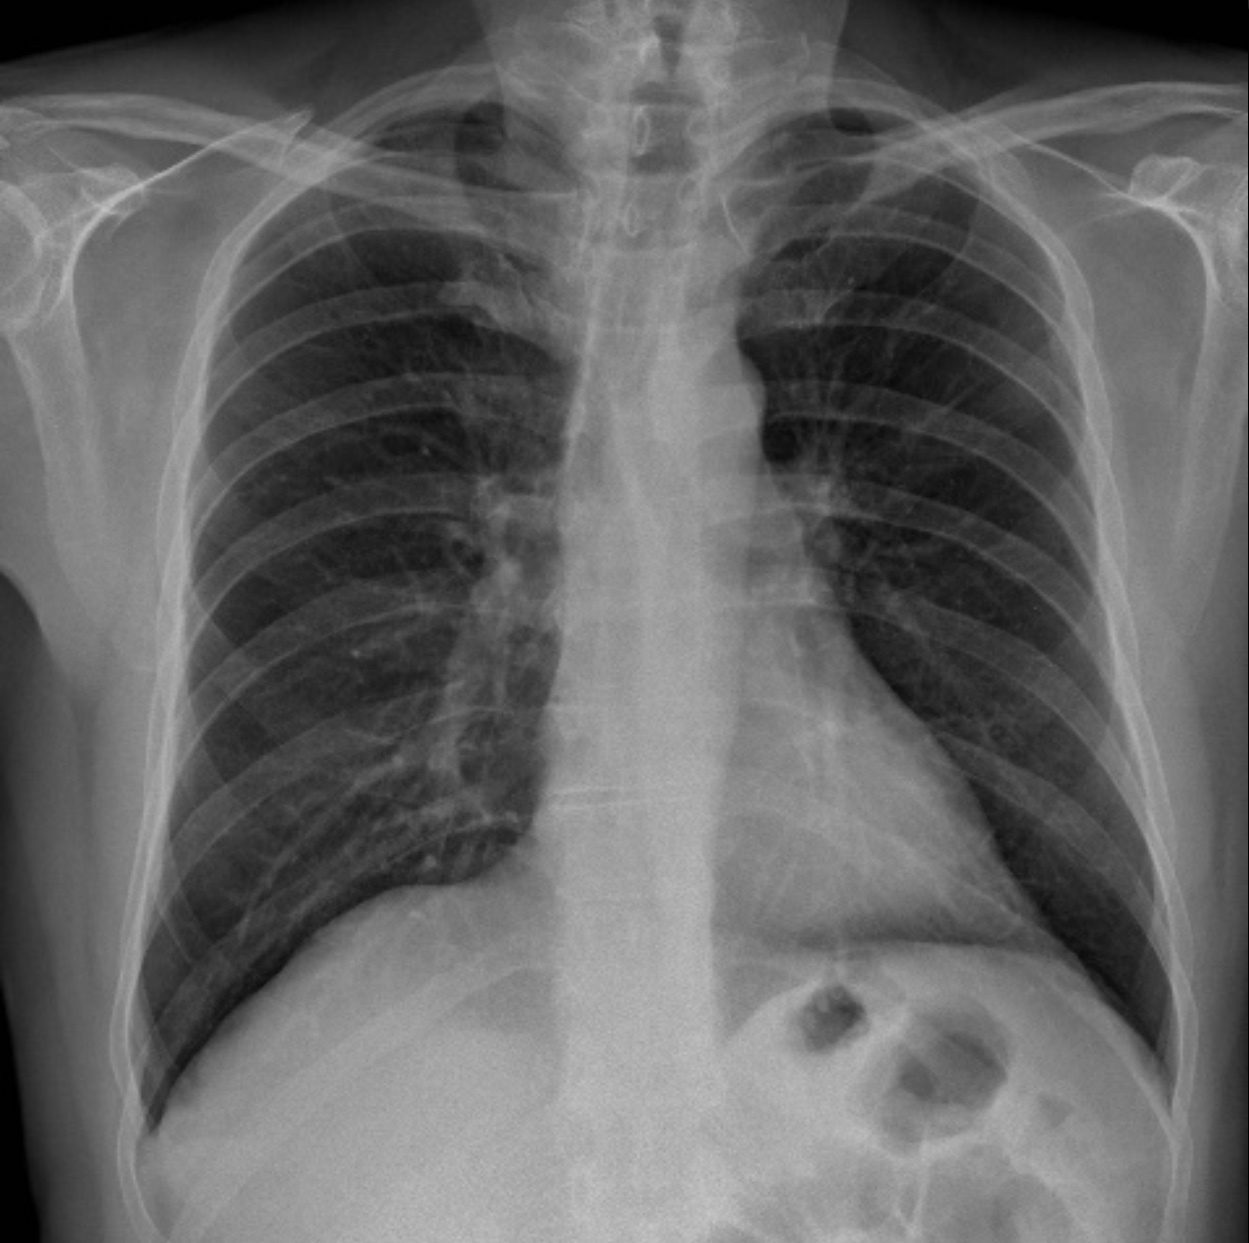
\includegraphics[width=\textwidth]{covid1.jpeg}
        \centering
        \caption{\textbf{Imagem original}}
        \label{fig:covid1antes}
    \end{subfigure}
    \hfill
    \begin{subfigure}[b]{0.45\textwidth}
        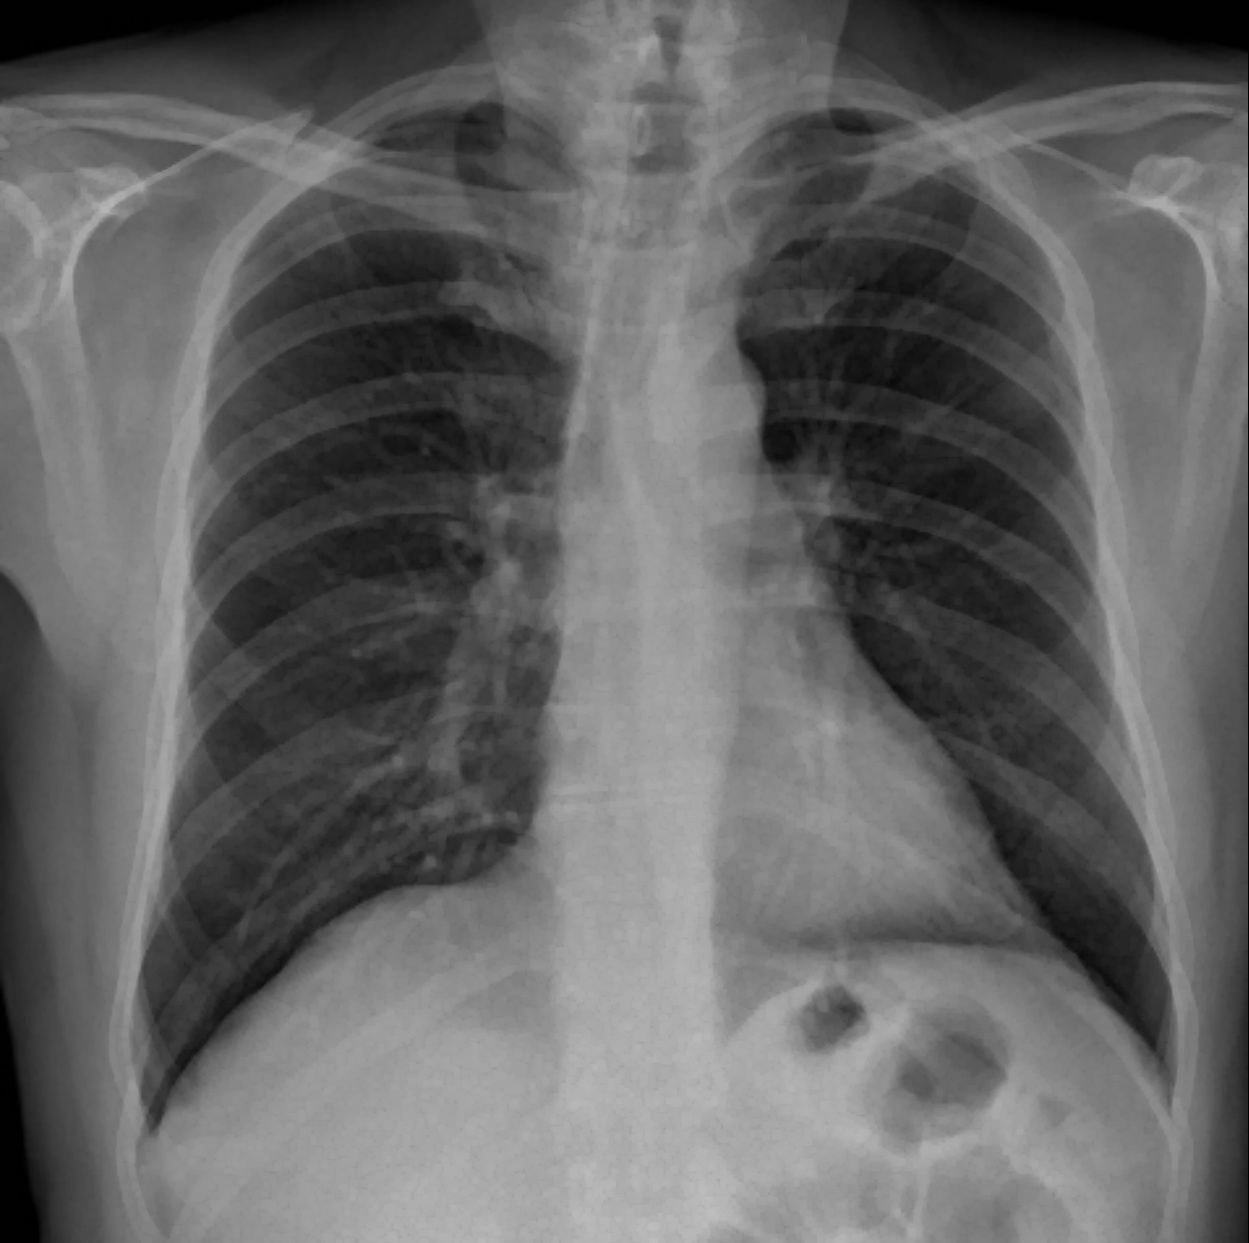
\includegraphics[width=\textwidth]{covid1opening.jpeg}
        \centering
        \caption{\textbf{{Imagem transformada}}}
        \label{fig:covid1opening}
    \end{subfigure}
    \caption{\textbf{{Imagem de COVID-19 antes e após a transformada de abertura.}}}
    \label{fig:covidopening}
\end{figure}

\begin{figure}[H]
\centering
    \begin{subfigure}[b]{0.45\textwidth}
        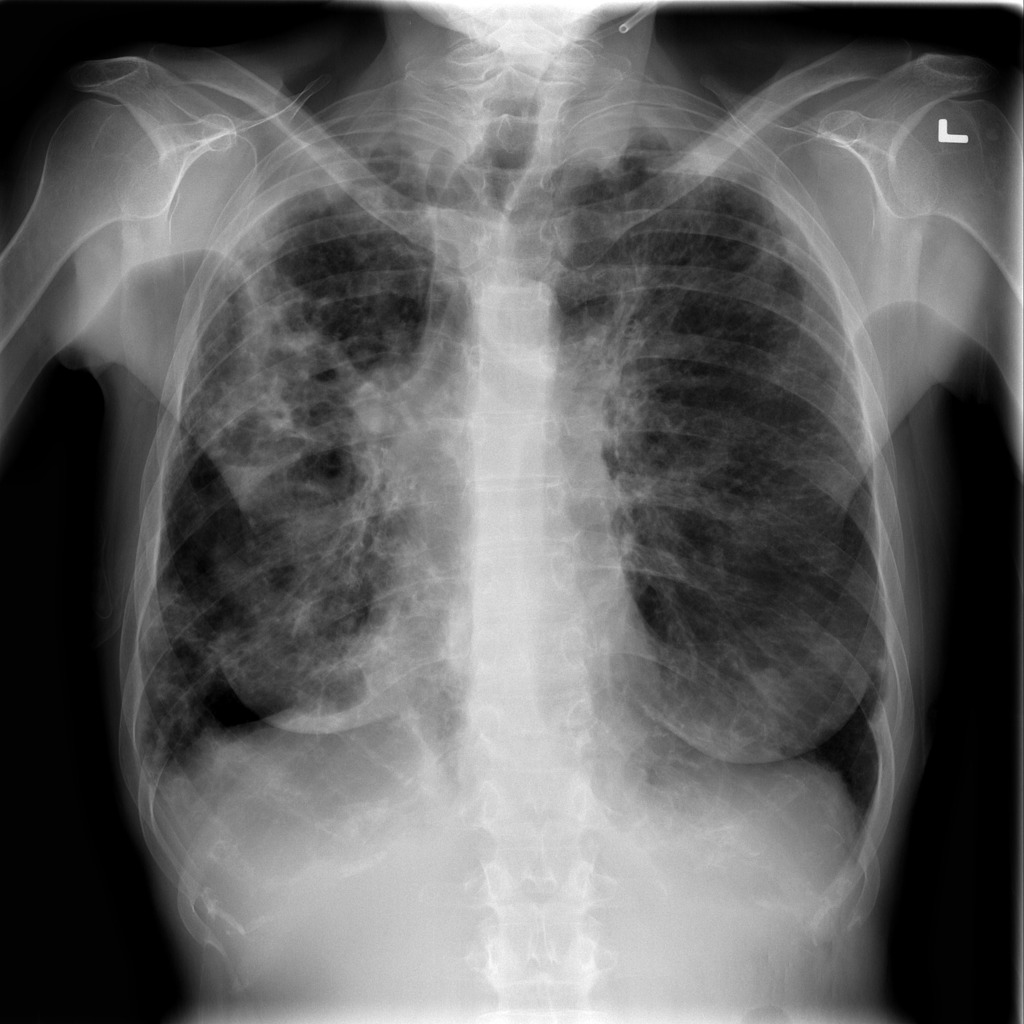
\includegraphics[width=\textwidth]{pneumo1.png}
        \centering
        \caption{\textbf{Imagem original}}
        \label{fig:pneumo1antes}
    \end{subfigure}
    \hfill
    \begin{subfigure}[b]{0.45\textwidth}
        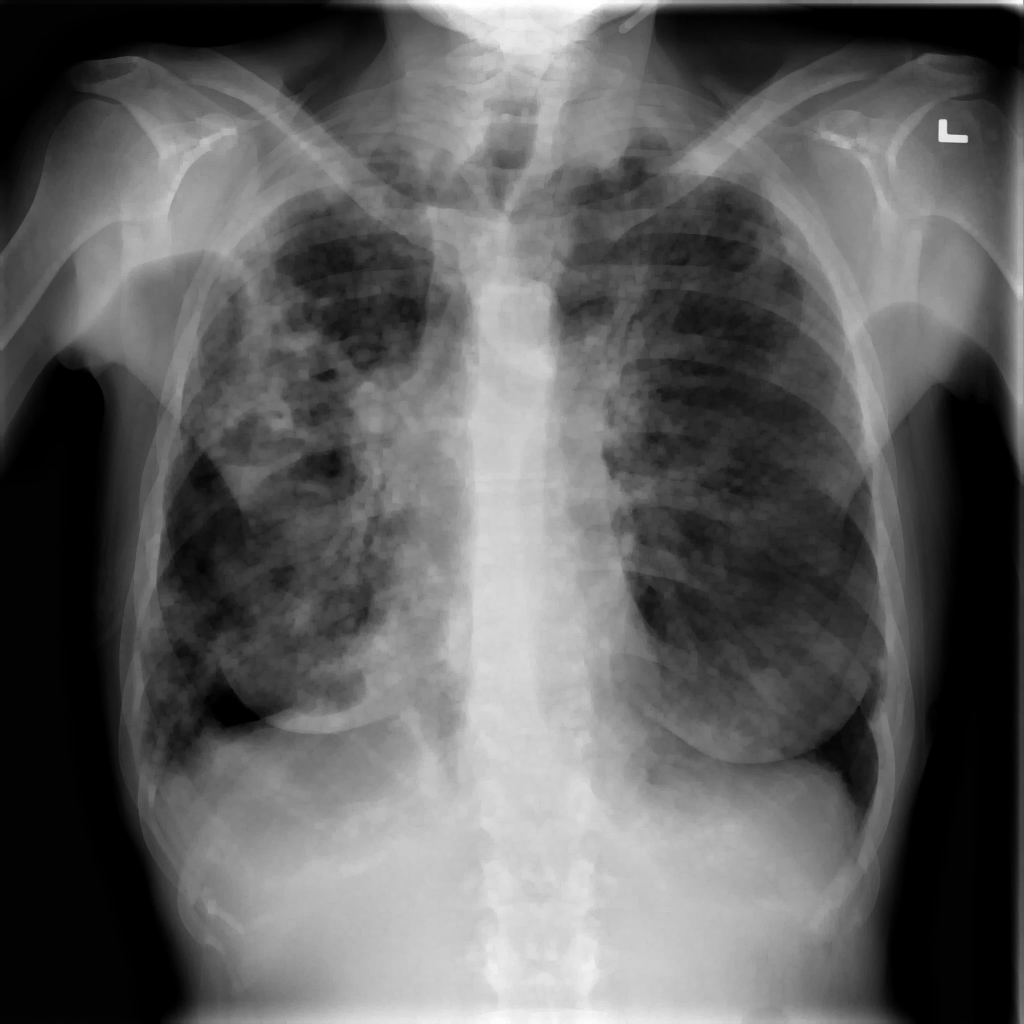
\includegraphics[width=\textwidth]{pneumo1opening.png}
        \centering
        \caption{\textbf{{Imagem transformada}}}
        \label{fig:pneumo1opening}
    \end{subfigure}
    \caption{\textbf{{Imagem de pneumonia antes e após a transformada de abertura.}}}
    \label{fig:pneumoopening}
\end{figure}

\begin{figure}[H]
\centering
    \begin{subfigure}[b]{0.45\textwidth}
        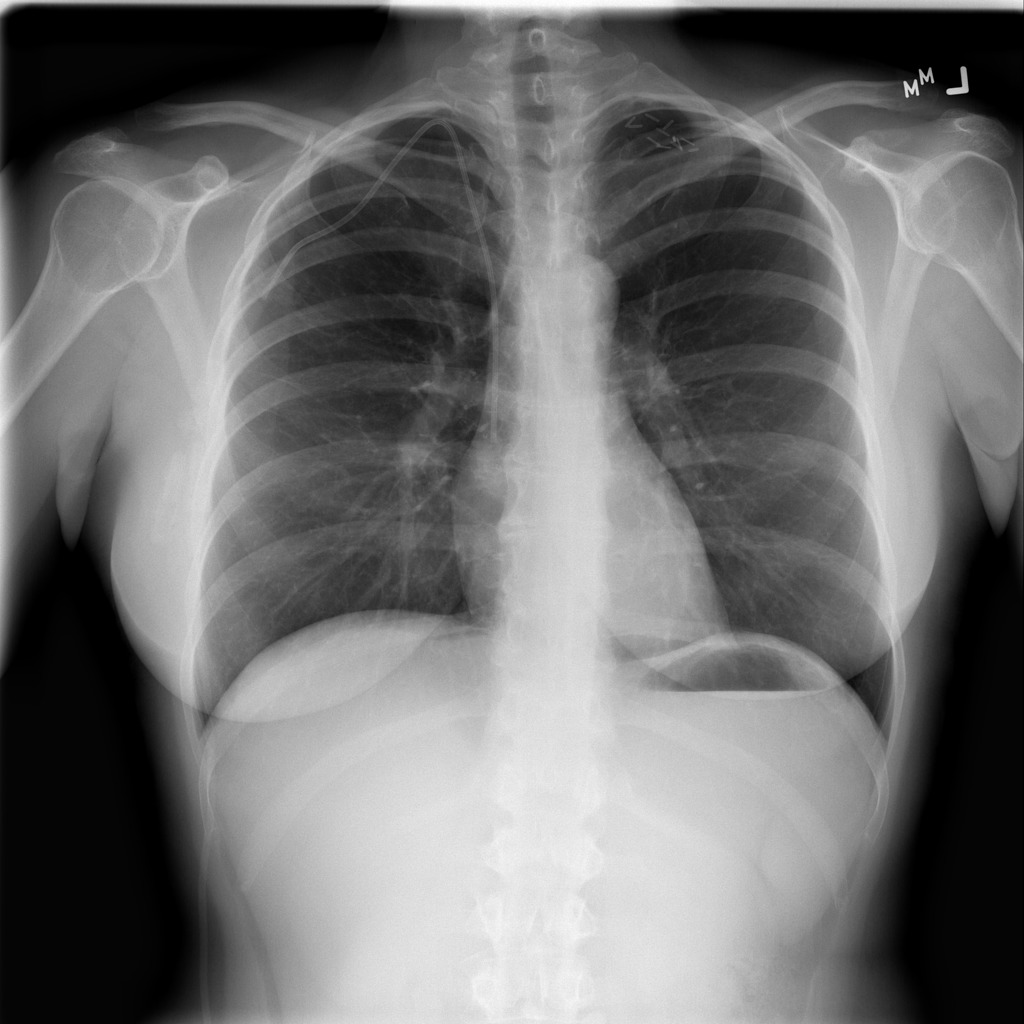
\includegraphics[width=\textwidth]{saudavel2.png}
        \centering
        \caption{\textbf{Imagem original}}
        \label{fig:saudavel2antes}
    \end{subfigure}
    \hfill
    \begin{subfigure}[b]{0.45\textwidth}
        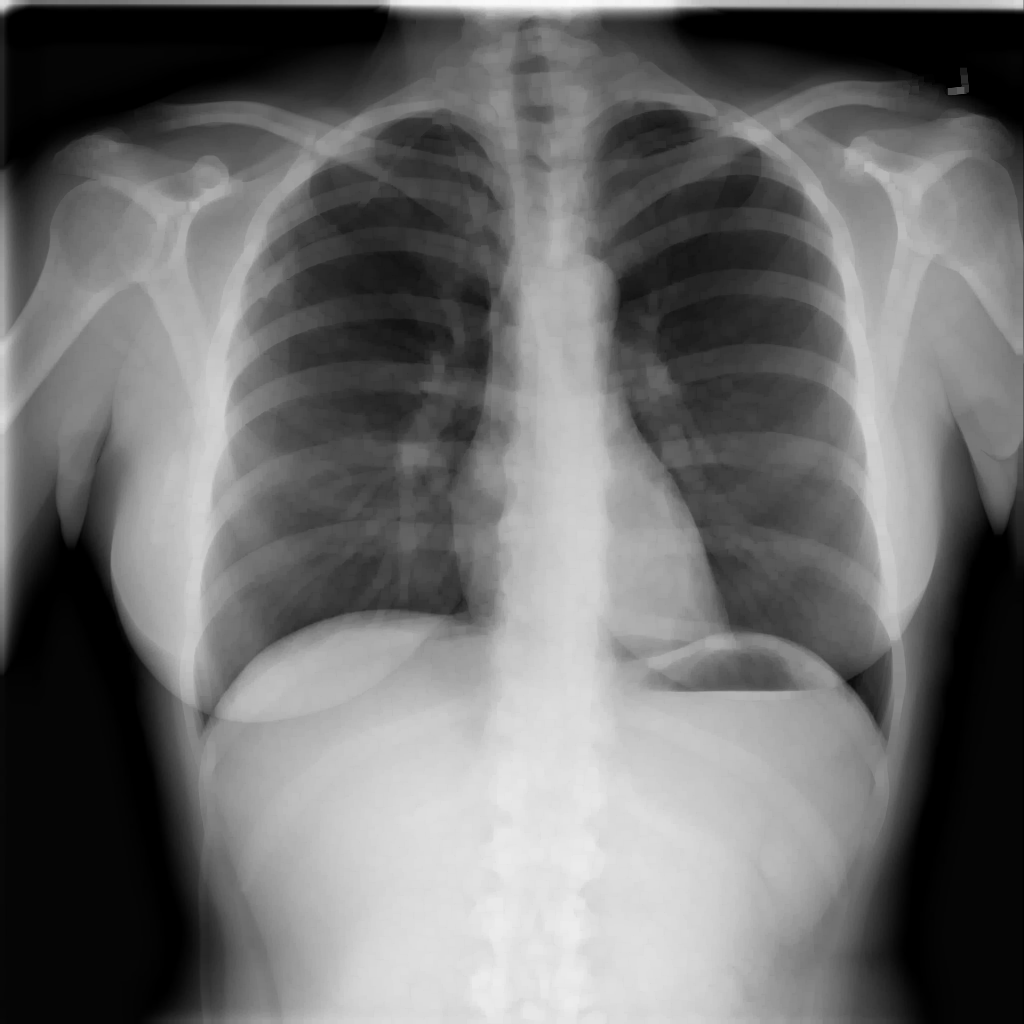
\includegraphics[width=\textwidth]{saudavel2opening.png}
        \centering
        \caption{\textbf{{Imagem transformada}}}
        \label{fig:saudavel2opening}
    \end{subfigure}
    \caption{\textbf{{Imagem de paciente saudável antes e após a transformada de abertura.}}}
    \label{fig:saudavelopening}
\end{figure}

\subsection{Classificação de Alto Nível Modificada}
Após aplicarmos a transformada morfológica abertura em nosso conjunto de imagens, convertemos cada imagem em uma vetor de características. Na montagem de nossa rede complexa, cada vetor de características que representa uma imagem original será um vértice e as ligações serão formadas por uma técnica que utiliza ora $K$ \textit{Nearest Neighbors}($K$NN), ora \textit{Radius Neighbors} (RN), buscando utilizar $K$NN para áreas esparsas e RN para áreas mais densas.

Para executar nossa técnica de classificação de alto nível, dividimos nosso conjunto de dados gerado em dois sub conjuntos, utilizando a proporção de 80\% e 20\%, de maneira aleatória e estratificada, ou seja, essa divisão foi realizada de maneira balanceada, mantendo a proporção amostras em cada classe entre os dois sub conjuntos. O primeiro conjunto de dados será utilizado para treinamento do nosso algoritmo e, o segundo, será para classificação, aferindo a eficiência do nosso classificador de alto nível.

Nosso conjunto de dados possui três classes: Saudável, pneumonia e COVID-19. Durante a fase de treinamento, nós calculamos três raios, um para cada classe. Esses raios serão utilizados pelo algoritmo \textit{Radius Neighbors}, o valor do raio será igual a média de todas as distâncias $K$NN dos componentes daquela classe no conjunto de dados de treinamento:

\begin{equation}
{R}={mean}(kNN_{dist}(X_{i},Y_{x_{i}}))
\end{equation}

Da mesma maneira, montamos três redes complexas, uma para cada classe e adicionamos componente a componente realizando sua ligação a outros componentes. Para as regiões mais esparsas, utilizamos os $K$ vizinhos mais próximos. Quando a quantidade de vizinhos dentro do raio $R$ for maior que o valor de $K$, nós criaremos uma ligação do nó para cada um dos seus $R$-vizinhos (vizinhos dentro do raio $R$). Dessa maneira, as ligações nas áreas densas e esparsas são determinadas segundo a seguinte fórmula:

\begin{equation}
    {V(x_{i})} = \begin{cases}{radiusNeighbors}(x_{i}, Y_{x_{i}}), {\ Se\ } | {radiusNeighbors}(x_{i}, Y_{x_{i}})| > K \\ {kNN} (x_{i}, Y_{x_{i}}), {\ Sen\tilde{a}o}\end{cases}
\end{equation}

onde $V_(x_{i})$ é o conjunto de vértices conectado com o vértice $x_i$, $kNN (x_{i}, Y_{x_{i}})$ é uma função que retorna o conjunto de $k$ vértices mais próximos e $radiusNeighbors(x_{i}, Y_{x_{i}})$ é uma função que retorna o conjunto de vértices dentro do raio $R$.

Na Figura~\ref{fig:rn}\index{Ilustração da metodologia de treinamento, onde a rede é formada por \textit{Radius Neighbor}} abaixo, ilustramos uma nova adição do vértice 10. Nesse exemplo, consideramos que o $K$ do algoritmo $K$NN é igual a três e que o $R$ na imagem se refere ao raio utilizado para o algoritmo RN. Dessa maneira, no exemplo a seguir, os nós 0, 1, 2, 4, 5 estão dentro do raio, totalizando cinco elementos. Como teríamos mais elementos no raio do que o valor de $K$, utilizaríamos o algoritmo \textit{Radius Neighbors} para adição do vértice 10, nesse caso seriam criados as seguintes arestas [(0, 10), (1, 10), (2, 10), (4, 10), (5, 10)]. A Figura~\ref{fig:rn}\index{Ilustração da metodologia de treinamento, onde a rede é formada por \textit{Radius Neighbor}} ilustra, então, uma área densa, na qual temos muitos elementos próximos, por isso, a utilização do RN para montagem da rede.

\begin{figure}[H]
    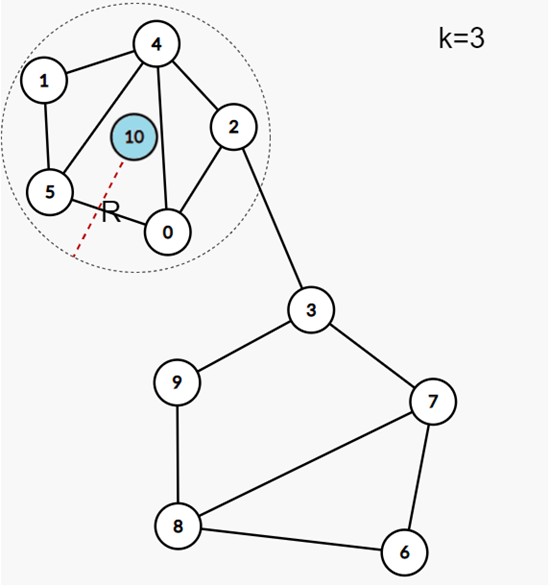
\includegraphics[scale=0.6]{rn.png}
    \centering
    \caption{\textbf{Exemplo de cenário onde seria utilizado o algoritmo \textit{Radius Neighbor} para montagem da rede.}}
    \label{fig:rn}
\end{figure}

Já na Figura~\ref{fig:knn}\index{Ilustração da metodologia de treinamento, onde a rede é formada por KNN} abaixo, ilustramos novamente a adição do vértice 10 em um novo posicionamento. Mais uma vez, consideramos que o $K$ do algoritmo $K$NN é igual a três e que o $R$ na imagem se refere ao raio utilizado para o algoritmo $R$-vizinhos. Nesse novo exemplo, apenas os nós 3 e 7 estão dentro do raio, totalizando dois elementos. Como nesse caso o valor de $K$ é superior a quantidade de elementos dentro do raio, nesse exemplo utilizaríamos o algoritmo $K$ \textit{Nearest Neighbors} para adição do vértice 10, nesse caso seriam criados as seguintes arestas [(3, 10), (7, 10)]. A Figura~\ref{fig:knn}\index{Ilustração da metodologia de treinamento, onde a rede é formada por $K$NN} ilustra uma área mais esparsa, onde temos poucos elementos próximos e esse foi o motivo da utilização do $K$NN para montagem da rede.

\begin{figure}[H]
    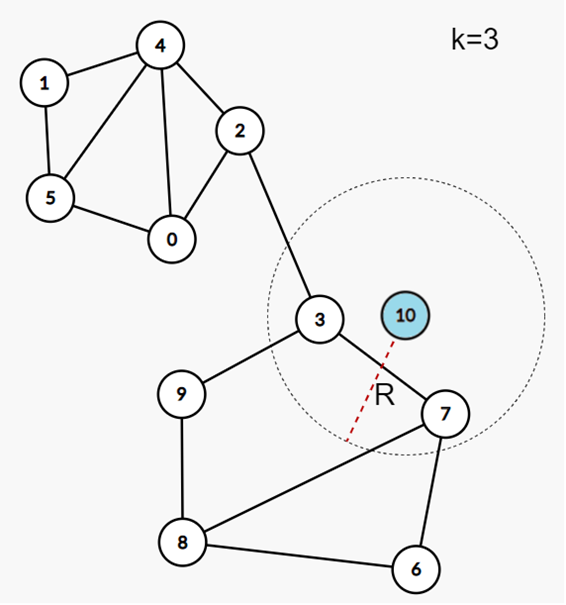
\includegraphics[scale=0.6]{knn.png}
    \centering
    \caption{\textbf{Exemplo de cenário onde seria utilizado o algoritmo k \textit{Nearest Neighbor} para montagem da rede.}}
    \label{fig:knn}
\end{figure}

Utilizando os conceitos anteriormente descritos vamos adicionando os membros um a um, seguindo a classe rotulada em $Y$. 
Após a construção da rede, a medida de cada rede, $G_{before} (class_i)$, $i = 1, 2, 3$, é calculada. Neste modelo, utilizamos a medida de comunicabilidade média $\langle M_{v_i} \rangle$ \cite{Estrada2008} sendo $G_{before, after} (class_i)$, que representa não apenas os caminhos mais curtos que conectam dois nós, mas também fazendo com que os caminhos mais longos tenham uma contribuição inferior a de caminhos mais curtos. O raciocínio por trás dessa escolha é que os caminhos mais curtos são significativamente afetados por mudanças estruturais em uma rede. 

Nos trabalhos anteriores \cite{silva2012a, Colliri2018}, um conjunto de medidas foi utilizado para caracterizar o padrão formado da rede, que introduz uma maior complexidade para determinação de pesos das medidas. Neste trabalho, propomos utilizar uma única medida (comunicabilidade), eliminando a necessidade da determinação de pesos e, ao mesmo tempo, apresentando uma precisão de classificação satisfatória.

Na fase de teste, utilizamos a mesma regra de inserção da fase de treinamento, ou seja, kNN para áreas esparsas e \textit{Radius Neighbors} para áreas mais densas e assim classificamos as amostras de dados não rotuladas uma a uma. Primeiramente, simulamos a inserção da nova amostra de dados em cada uma das três redes construídas até o momento. Então, a medida de comunicabilidade de cada rede após a inserção, $G_{after} (class_i)$, $i = 1, 2, 3$ é calculada. 
Assim, obtemos o impacto da inserção da nova amostra para cada classe.

\begin{equation}
\Delta G (class_i) = || G_{before} (class_i) - G_{after} (class_i) ||, i = 1,2,3.
\end{equation}

Finalmente, a nova amostra é classificada na classe $j$, onde 
\begin{equation}
\Delta G (class_j) = min \{\Delta G (class_i) \}, i = 1,2,3.
\end{equation}

Em outras palavras, a nova amostra terá conformidade com o padrão formado pela rede $j$ se não produzir perturbação significante à rede $j$. A amostra, então, é inserida de fato à rede $j$, onde foi classificada. Observe que a nova amostra pode até ficar longe dos elementos da classe $j$, o que pode ser um problema para alguns classificadores de baixo nível, mas como o nosso classificador de alto nível se baseia padrões ao invés de distância, então, ele classificará corretamente.



\chapter{Resultados Experimentais}
Neste capítulo serão apresentados os resultados obtidos com nosso classificador de alto nível e com um caráter de linha de base utilizamos também outros classificadores tradicionais. Na primeira seção, classificaremos dados artificias, já na segunda seção, classificaremos dados reais, ou seja, as imagens de raio X de pacientes com COVID-19, pneumonia e saudáveis.

\section{Conjuntos de dados artificiais}
Para testar nosso classificador de alto nível, realizamos, primeiramente, um teste em um conjunto de dados artificial produzido pelo algoritmo \textit{make moons} \cite{scikit-learn}. Esse algoritmo gera amostras que quando distribuídas em um plano cartesiano forma dois semicírculos intercalados. Por meio desse algoritmo, geramos um conjunto de dados composto com 500 amostras, conforme ilustra a Figura~\ref{fig:artificial_moons}\index{conjunto de dados \textit{Moons} com quinhentas amostras.}. 

\begin{figure}[H]
    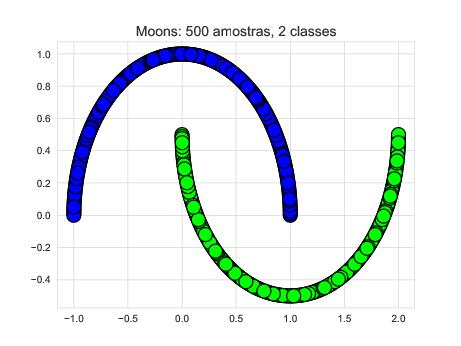
\includegraphics[scale=0.6]{artificial_moons.png}
    \centering
    \caption{\textbf{Conjunto de dados \textit{Moons} com quinhentas amostras.}}
    \label{fig:artificial_moons}
\end{figure}

Esse conjunto foi subdividido em dois subconjuntos, utilizando a proporção de 80\% e 20\%, também de maneira aleatória e estratificada. O primeiro conjunto de dados será utilizado para treinamento do nosso algoritmo e, o segundo, será para classificação, aferindo a eficiência do nosso classificador de alto nível. Nessa execução, utilizamos o valor de \textit{K}=2, o atributo \textit{K} se refere a quantidade de vizinhos utilizados no kNN para montagem da rede. Após a fase de treinamento, duas redes foram criadas, elas estão ilustradas nas Figuras~\ref{fig:moons0}\index{Rede resultante do treinamento para da primeira classe do conjunto de dados \textit{Moon}.} e~\ref{fig:moons1}\index{Rede resultante do treinamento para da segunda classe do conjunto de dados \textit{Moon}.}. As cores dos vértices representam o seu grau, ou seja, a quantidade de arestas conectadas a esse vértice. Os tons mais claros de azul representam um grau menor, enquanto os tons mais escuros representam um grau maior. A tonalidade mais clara do azul equivale ao valor de $K$, nesse caso 2, dessa maneira, conseguimos visualizar onde o algoritmo utilizou kNN e onde ele utilizou \textit{Radius Neighbors}, sempre que o grau for igual ao número de $K$ a inserção terá sido realizada através dos K vizinhos mais próximos e todas as vezes que ele for maior o algoritmo utilizado terá sido dos vizinhos dentro do raio. Podemos notar que os vértices periféricos quase em sua totalizada possuem a tonalidade mais clara de azul, ou seja, foram inseridos por kNN. Vemos graus maiores nas regiões centrais das redes, indicando um padrão de distribuição e consequentemente um padrão de preferência na rede.

\begin{figure}[H]
\centering
    \begin{subfigure}[b]{0.49\textwidth}
        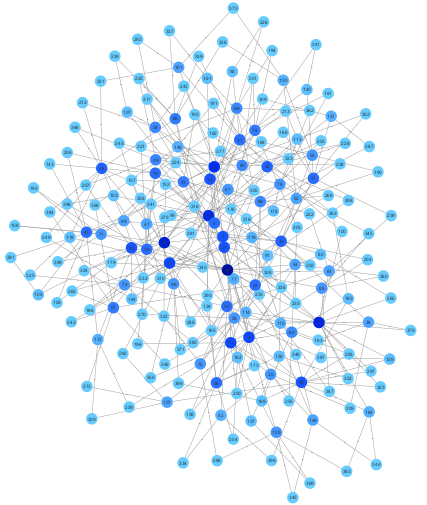
\includegraphics[width=\textwidth]{moons0.png}
        \centering
        \caption{\textbf{Rede primeira classe}}
        \label{fig:moons0}
    \end{subfigure}
    \hfill
    \begin{subfigure}[b]{0.49\textwidth}
        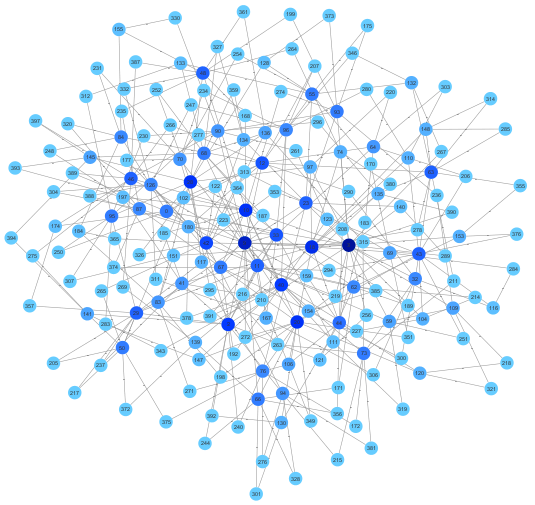
\includegraphics[width=\textwidth]{moons1.png}
        \centering
        \caption{\textbf{{Rede segunda classe}}}
        \label{fig:moons1}
    \end{subfigure}
    \caption{\textbf{{Redes resultantes do treinamento do conjunto de dados gerado pelo \textit{make moons}.}}}
    \label{fig:moons}
\end{figure}

Para mensurar o desempenho de nosso classificador de alto nível, realizamos o treinamento e classificação também em diversos classificadores de baixo nível. Os classificadores utilizados foram: \textit{AdaBoost, Bagging Decision Tree, Bagging SVC, Decision Tree, K Nearest Neighbors, Logistic Regression, Multilayer Perceptron, Naive Bayes Bernoulli, Naive Bayes Gaussian, Naive Bayes Multinomial, Radius Neighbors, Random Forest, SVM}, além disso, replicaremos o resultado obtido na pesquisa de \cite{Colliri2018}. Nós utilizamos a implementação padrão desses algoritmos contidas na biblioteca scikit-learn \cite{scikit-learn} e obtivemos os resultados ilustrados na Tabela~\ref{tab:resultadomoon1}.

\begin{table}[ht]
\caption{Comparativo dos desempenhos de diversos classificadores e do nosso classificador de alto nível no conjunto de dados \textit{Moon} sem ruído.}
\label{tab:resultadomoon1}
  \centering
\begin{tabular}{l|c}\hline
 Classificador & Resultado\\\hline
AdaBoost & 100\% \\ 
Bagging Decision Tree & 100\% \\ 
Bagging SVC with SVC & 100\% \\ 
BernoulliNB & 80\% \\
Decision Tree & 100\% \\
GaussianNB & 89\% \\ 
KNN & 100\% \\ 
Logistic Regression & 90\% \\
MultiLayer Perceptron & 94\% \\ 
NBHL \cite{Colliri2018} & 100\% \\
Radius Neighbors & 45\% \\
RandomForestClassifier & 91\% \\ 
SVM & 100\% \\
\textbf{Classificador de alto nível proposto} & 100\% \\\hline
\end{tabular}
\end{table}

O conjunto de imagens \textit{moon} possui uma clara distribuição das amostras, o que facilita a classificação precisa dos algoritmos. Para incrementar a dificuldade e sobrepor algumas amostras, aplicamos um fator de ruído na criação do conjunto de dados \textit{moon}. Esse fator fez com que o padrão visual, antes bem separado, passasse a ser não tão facilmente reconhecido. A Figura~\ref{fig:artificial_moons_noise}\index{Conjunto de dados \textit{Moons} com quinhentas amostras e fator de ruído 0.25.}, ilustra a distribuição das amostras em um plano cartesiano.

\begin{figure}[H]
    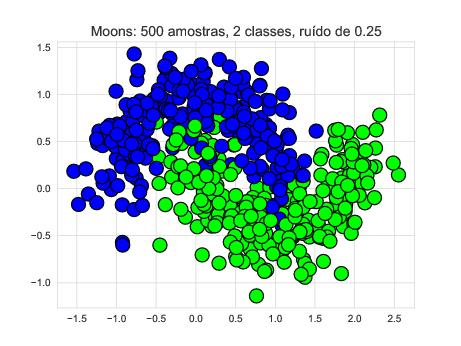
\includegraphics[scale=0.6]{artificial_moons_noise.png}
    \centering
    \caption{\textbf{Conjunto de dados \textit{Moons} com quinhentas amostras e fator de ruído 0.25.}}
    \label{fig:artificial_moons_noise}
\end{figure}

Esse novo conjunto incrementa a complexidade, já que não é tão bem dividido a distribuição de cada classe. Utilizamos o valor de \textit{K}=2 para mensurar o desempenho de nosso classificador de alto nível. Realizamos o treinamento e classificação nos mesmos algoritmos do problema anterior, utilizando as mesmas implementações e parâmetros e obtivemos os resultados ilustrados na Tabela~\ref{tab:resultadomoon2}.

\begin{table}[ht]
\caption{Comparativo dos desempenhos de diversos classificadores e do nosso classificador de alto nível no conjunto de dados \textit{Moon} com ruído 0.25.}
\label{tab:resultadomoon2}
  \centering
\begin{tabular}{l|c}\hline
 Classificador & Resultado\\\hline
AdaBoost & 92\% \\ 
Bagging Decision Tree & 94\% \\ 
Bagging SVC with SVC & 92\% \\ 
BernoulliNB & 76\% \\
Decision Tree & 92\% \\
GaussianNB & 84\% \\
KNN & 92\% \\ 
Logistic Regression & 84\% \\
MultiLayer Perceptron & 88\% \\ 
NBHL \cite{Colliri2018} & 96\% \\
Radius Neighbors & 45\% \\
RandomForestClassifier & 86\% \\ 
SVM & 92\% \\
\textbf{Classificador de alto nível proposto} & 95\% \\\hline
\end{tabular}
\end{table}

\section{Conjuntos de dados reais}
Nosso classificador se comportou bem para solucionar um problema artificial, tendo uma ótima acurácia. Por último, realizamos a execução do nosso classificador de alto nível em um problema real, a identificação de imagens de raio-x de pacientes com COVID-19, Pneumonia e saudáveis. Para isso, utilizamos valores de \textit{k} entre um e cinco. O melhor desempenho foi obtido utilizando também \textit{K}=2. Dessa maneira, antes de mostrar os resultados de classificação, vamos visualizar as redes geradas na fase de treinamento utilizando o k=2. As Figuras~\ref{fig:rede0}\index{Rede de treinamento da classe COVID-19},~\ref{fig:redereduzida1}\index{Rede de treinamento da classe Pneumonia} e~\ref{fig:redereduzida2}\index{Rede de treinamento da classe de pacientes saudáveis} mostram cada uma das redes geradas após a fase de treinamento, a primeira imagem é da rede formada por membros da classe COVID-19, a segunda é da rede de membros com Pneumonia, e a terceira é da rede formada por indivíduos saudáveis. Buscando melhorar a visualização, destacamos a cor dos nós de maneira gradiente, considerando o grau de cada vértice, nos quais as cores mais claras significam um menor grau, ou seja, menos conexões, e as cores mais escuras representam um número maior de conexões. O azul mais claro equivale ao valor de \textit{K}, dessa maneira, podemos visualizar quais vértices foram inseridos utilizando kNN e quais foram inseridos utilizando \textit{radius neighbors}. Podemos notar uma clara preferência por alguns nós da rede e essa formação contribui para que a comunicabilidade retorne padrões diferentes para cada rede. É possível visualizar que cada rede possui um padrão visual, corroborando com os conceitos de nosso método.

\begin{figure}[H]
    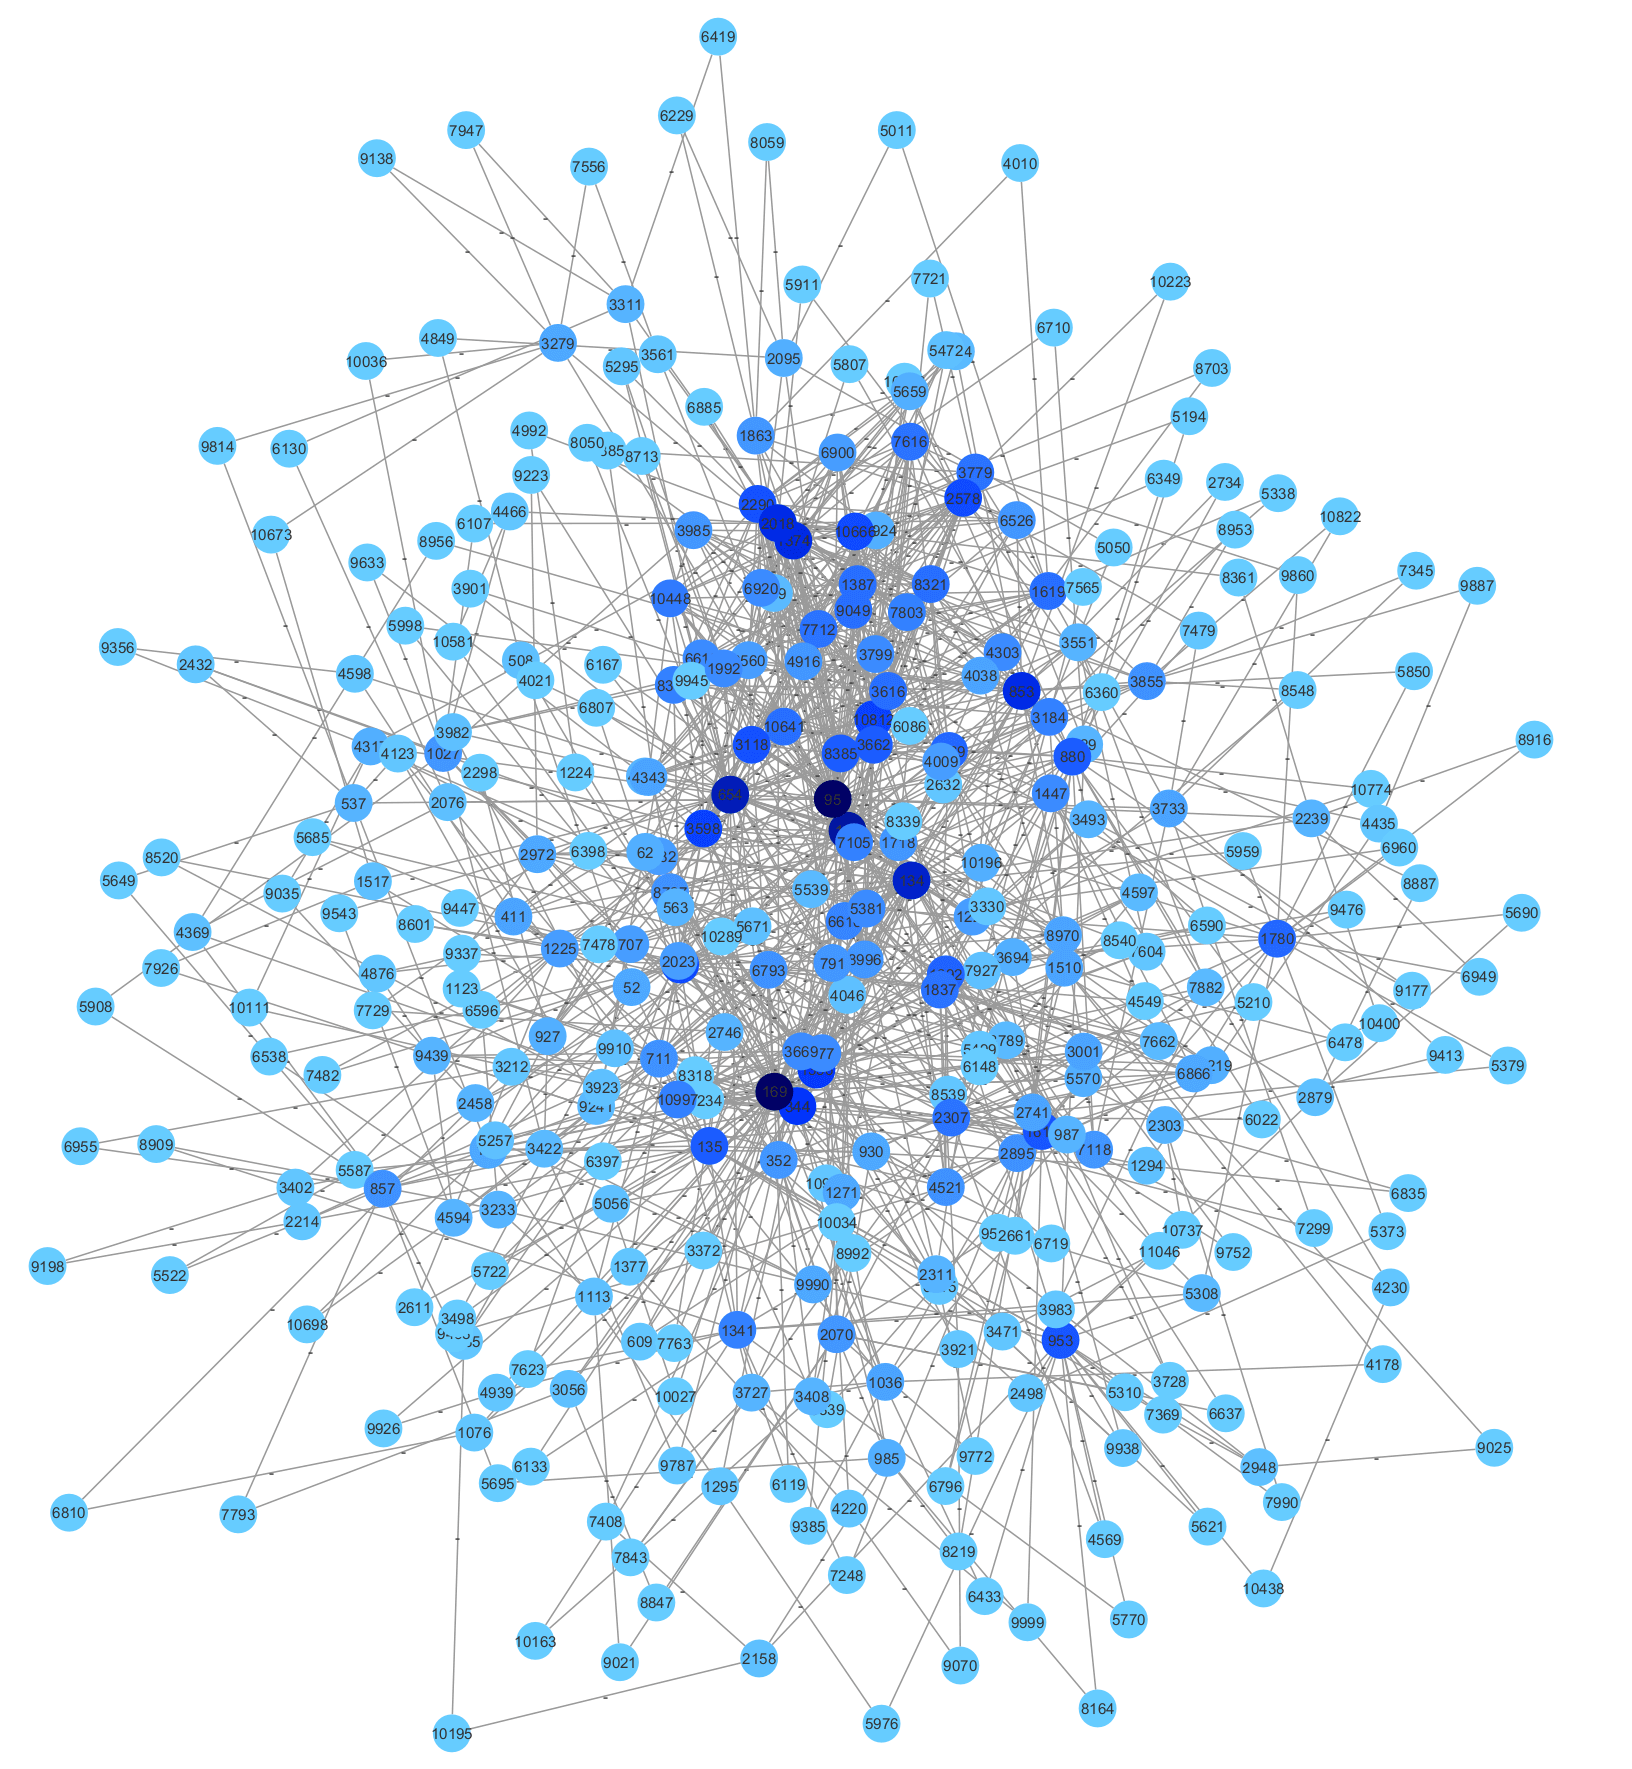
\includegraphics[width=\textwidth]{rede0.png}
    \centering
    \caption{\textbf{Rede resultante do treinamento para a classe de COVID-19.}}
    \label{fig:rede0}
\end{figure}

\begin{figure}[H]
    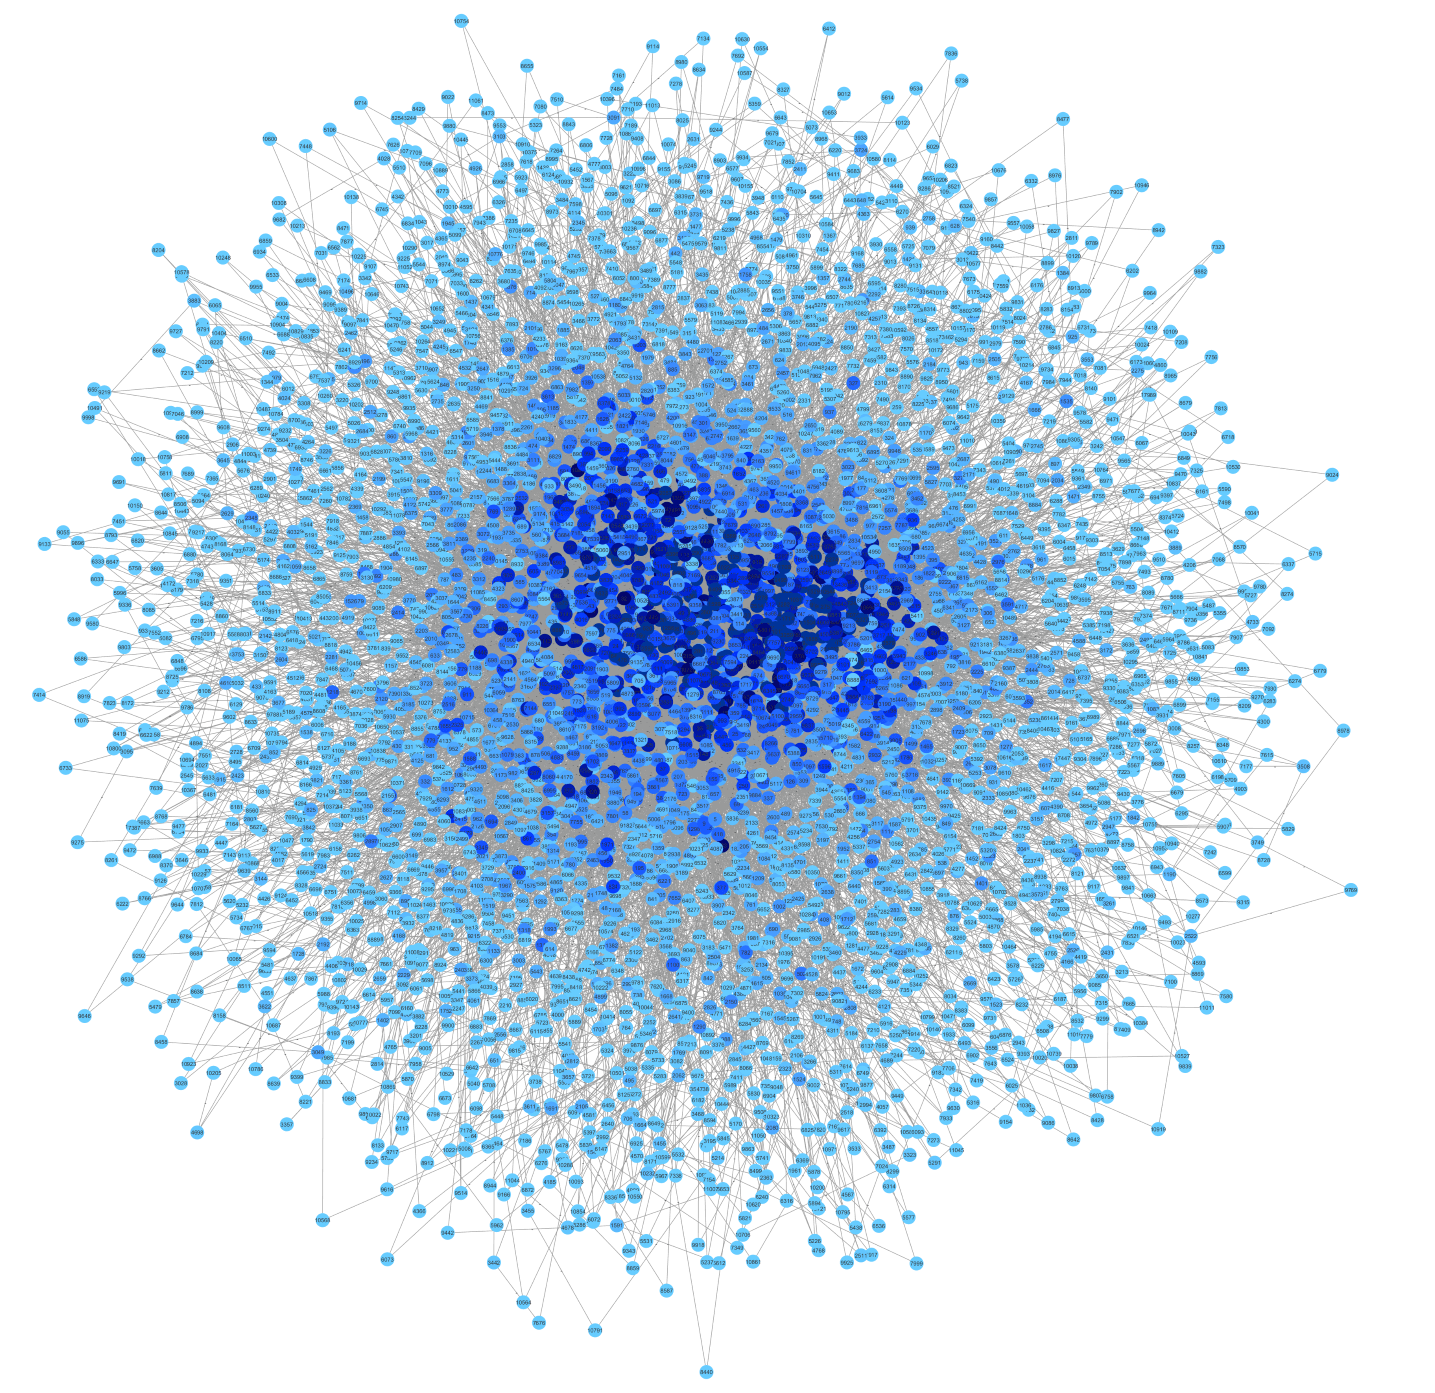
\includegraphics[width=\textwidth]{redereduzida1.png}
    \centering
    \caption{\textbf{Rede resultante do treinamento para a classe de Pneumonia.}}
    \label{fig:redereduzida1}
\end{figure}

\begin{figure}[H]
    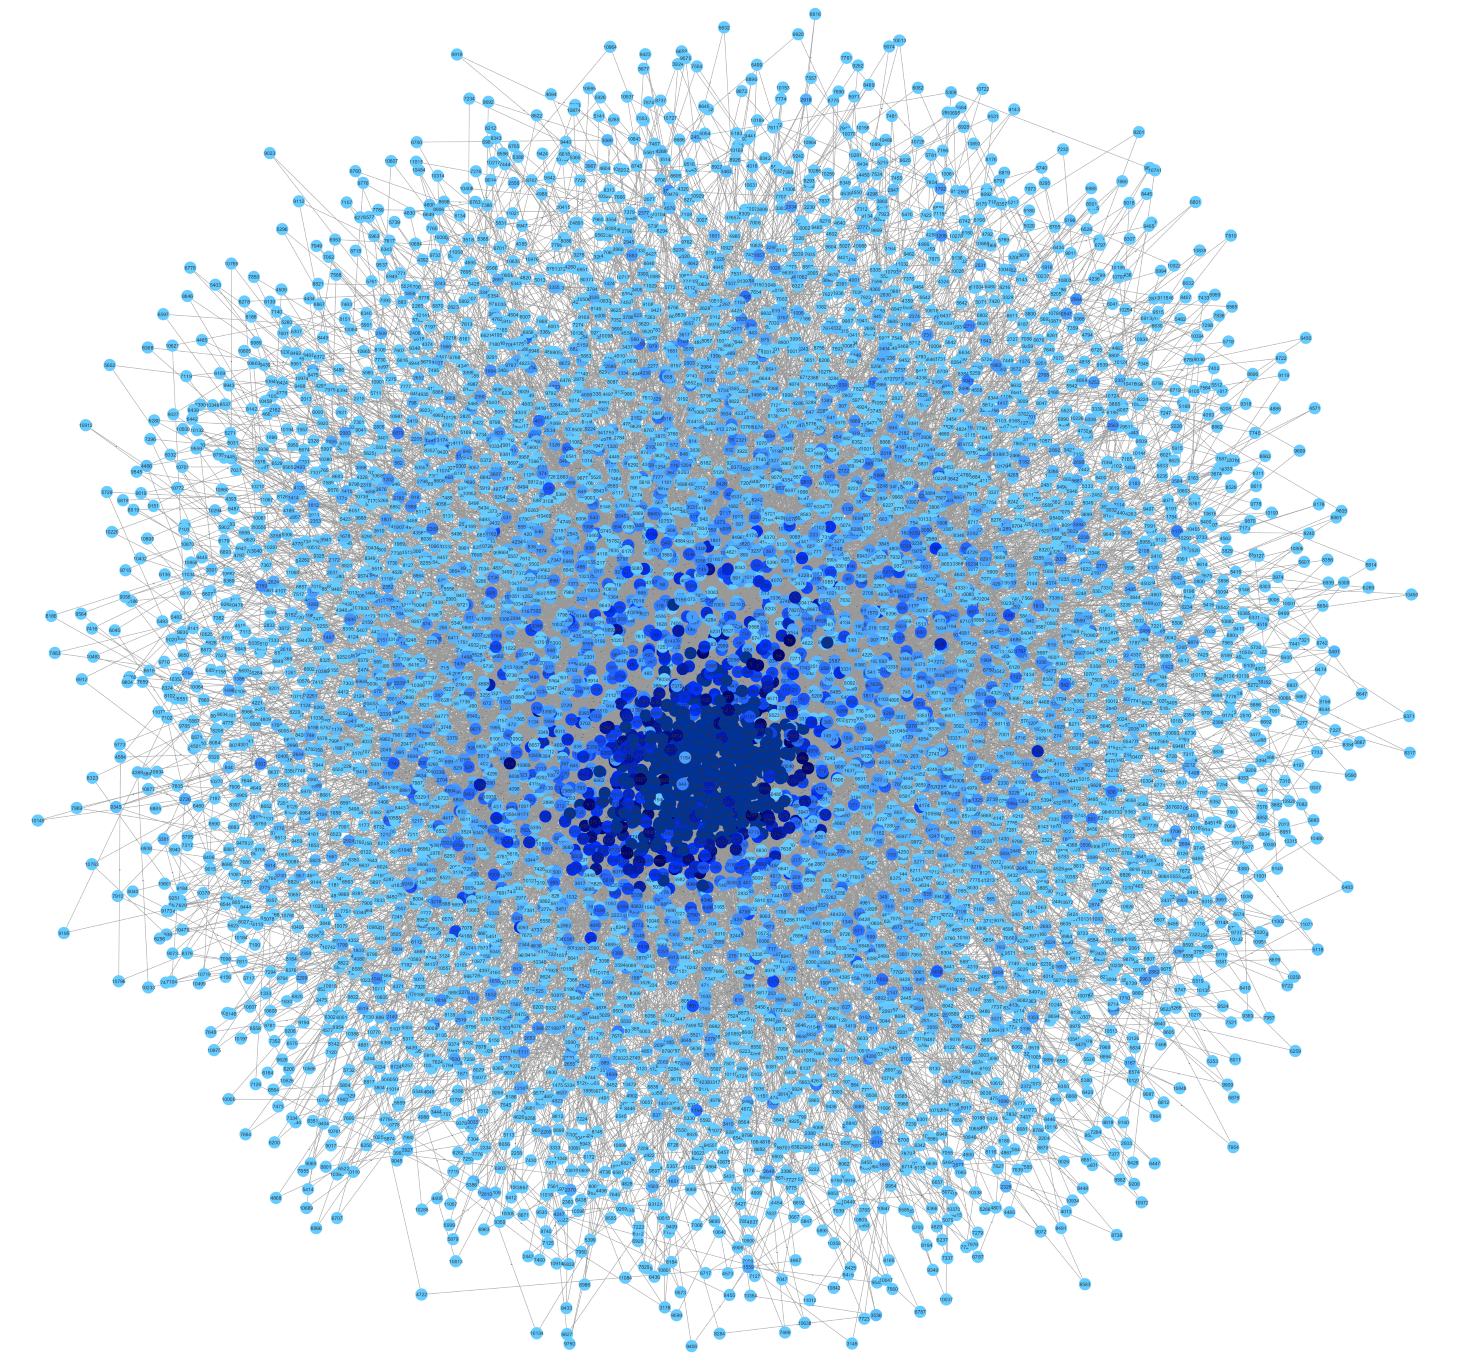
\includegraphics[width=\textwidth]{redereduzida2.png}
    \centering
    \caption{\textbf{Rede resultante do treinamento para a classe de pessoas saudáveis.}}
    \label{fig:redereduzida2}
\end{figure}

Apesar de obtermos um melhor resultado com um determinado $K$, notamos que a diferença de acurácia em grandes redes não se altera de maneira significativa com a alteração do valor de $K$. Aparentemente, isso se deve ao fato da utilização de dois algoritmos para montagem da rede, além disso, conforme a rede cresce a preferência por determinados nós fazem com que o grau de alguns vértices seja superior a trinta vezes o valor do $K$ máximo que utilizamos, ou seja, conforme a rede cresce, ela passa a ter nós com grau superior a 150. Mesmo na rede do COVID-19, que possui muito menos amostras, possuímos nós com grau acima de 50. Notamos também que a escolha por definir um valor de $R$ (raio) para cada rede, ou seja, para cada classe, ao invés de um $R$ único valor fortalece ainda mais a distinção de padrões entre as redes. Com um raio para cada rede, garantimos que sempre sera utilizado \textit{radius neighbors} quando houver mais vizinhos do que o valor de \textit{K}, utilizando um raio para as três redes nem sempre isso ocorrerá. Em testes, a acurácia foi incrementada em aproximadamente 2\% ao utilizar um raio para cada rede. 

Para mensurar o desempenho de nosso classificador de alto nível, realizamos o treinamento e classificação também em diversos classificadores de baixo nível. Os classificadores utilizados foram: \textit{AdaBoost, Bagging Decision Tree, Bagging SVC, Decision Tree, K Nearest Neighbors, Logistic Regression, Multilayer Perceptron, Naive Bayes Bernoulli, Naive Bayes Gaussian, Naive Bayes Multinomial, Radius Neighbors, Random Forest e SVM}. Nós utilizamos a implementação padrão desses algoritmos contida na biblioteca \textit{scikit-learn} \cite{scikit-learn} e obtivemos os resultados ilustrados na Tabela~\ref{tab:resultado}, já na Tabela~\ref{tab:resultadoreport} mostramos a Precisão, a revocação e o F1-score do nosso classificador de alto nível.

\begin{table}[h]
\caption{Comparativo dos desempenhos de diversos classificadores e do nosso classificador de alto nível no conjunto de imagens de raio-x.}
\label{tab:resultado}
  \centering
\begin{tabular}{l|c|c}\hline
 Classificador & Resultado & F1-score COVID-19\\\hline
AdaBoost & 80,59\% & 0,47\\
Bagging Decision Tree & 80,92\% & 0,23\\
Bagging SVC & 84,63\% & 0,38\\
Decision Tree & 74,39\% & 0,20\\
K Nearest Neighbors & 79,12\% & 0,44\\
Logistic Regression & 81,60\% & 0,46\\
Multilayer Perceptron & 83,95\% & 0,26\\
Naive Bayes Bernoulli & 57,51\% & 0,02\\
Naive Bayes Gaussian & 67,03\% & 0,18\\
Naive Bayes Multinomial & 64,04\% & 0,18\\
Radius Neighbors & 63,36\% & 0,0\\
Random Forest & 79,33\% & 0,0\\
SVM & 84,41\% & 0,43\\
\textbf{Classificador de alto nível proposto} & 90,6\% & 0,85\\\hline
\end{tabular}
\end{table}

\begin{table}[h]
\caption{Precisão, revocação e F1-score do nosso classificador de alto nível.}
\label{tab:resultadoreport}
  \centering
\begin{tabular}{l|c|c|c}\hline
& Precisão & Revocação & f1-score\\
COVID-19 & 0,806 & 0,908 & 0,854\\
Pneumonia & 0,891 & 0,870 & 0,880\\
Saudável & 0,923 & 0,931 & 0,927\\\hline
\end{tabular}
\end{table}


Conforme demonstrado nas tabelas, nosso algoritmo se mostrou superior aos classificadores tradicionais para identificar imagens do novo corona vírus. Isso se deve ao fato dele conseguir encontrar padrões entre as classes ao invés de utilizar apenas aspectos físicos.

Para certificar como o nosso classificador de alto nível se comportaria diante de um novo conjunto de imagens, realizamos o download no repositório tawsifurrahman \cite{repo5} do conjunto de imagens de pacientes que contraíram o SARS-CoV-2. Este repositório conta com 219 imagens de COVID-19, e utilizando nosso algoritmo, já treinado anteriormente, classificamos essas novas imagens. Nesse cenário, o nosso classificador obteve um resultado preditivo ainda melhor, contabilizando 91.4\% de acurácia.

Existem alguns outros grandes trabalhos de pesquisa utilizando inteligência artificial para detecção de COVID-19 em imagens médicas. Um dos mais relevantes é o COVID-Net, no qual eles utilizam uma \textit{deep convolutional neural network} para a classificação das imagens. Em sua primeira pesquisa publicada, eles possuíam um índice de 80\% de acerto para imagens de COVID-19, atualmente, o projeto conseguiu uma acurácia de 93,3\% e uma sensibilidade de 91,0\%\cite{wang2020covidnet}, segundo algoritmo disponível do \textit{GitHub} do autor \cite{covidnet}. Um resultado não tão distante do obtido em nossa pesquisa.


% ----------------------------------------------------------
% Finaliza a parte no bookmark do PDF
% para que se inicie o bookmark na raiz
% e adiciona espaço de parte no Sumário
% ----------------------------------------------------------
\phantompart

% ---
% Conclusão
% ---
\chapter{Conclusão e Trabalhos Futuros}

Os resultados obtidos neste trabalho fazem uma relevante contribuição para a área de aprendizado de máquina e, principalmente, para o combate da pandemia. Apresentaremos, a seguir, um resumo das principais realizações desse trabalho.

\section{Principais Contribuições}

A dissertação demonstrou a possibilidade de extrair padrões de imagens de raio-x a partir da montagem de uma rede complexa e da análise de impactos em medidas dessa rede. O desenvolvimento de um algoritmo de classificação de alto nível utilizando esses conceitos contribui ainda para a área do saber de aprendizado de máquina e classificadores. 

A acurácia superior do método proposto, comparada às técnicas de classificação de dados tradicionais, comprova que a identificação de padrões é uma maneira eficiente para predição de classes, e que, em diversos cenários, ela pode ser superior a de características físicas.

A comunicabilidade se mostrou uma métrica capaz de identificar e de extrair características necessárias para a classificação de imagens de COVID-19. Dessa maneira, o classificador de alto nível se mostra promissor na resolução do problema de classificação de imagens médicas de COVID-19.

Utilizar uma medida de raio para cada classe da rede consegue melhorar o algoritmo de montagem da rede utilizando as técnicas de kNN e radius neighbors.

Considerando que outros trabalhos utilizaram redes para solução de outros problemas e também para outros tipos de classificação e que obtiveram também bons resultados aplicando esse conceito, concluímos que a técnica pode ser utilizada com sucesso para diferentes finalidades, permitindo solucionar diversos problemas nos quais existem padrões sobrepostos\cite{silva2012a, Colliri2018}.


\section{Melhorias e Trabalhos Futuros}

O algoritmo apesar de ter se mostrado eficiente, demanda de um grande poder computacional e, consequentemente, requer um longo tempo para processamento, tanto no momento de treinamento quanto no momento de classificação. O problema de performance é ainda mais agravado com o crescimento da rede, pois os cálculos se tornam mais complexos e mais dispendiosos.

Como melhorias, buscaremos em trabalhos futuros, otimizar o código de maneira que esse tempo possa ser reduzido. Almeja-se, também, buscar uma maneira de realizar um pré-processamento no qual as características e padrões não sejam perdidos, possibilitando reduzir o tempo, porém sem afetar os resultados.

Será implementado técnicas para extrair apenas os pulmões nas imagens e, assim, garantir uma comparação mais precisa entre imagens de diferentes repositórios.

Serão testado algoritmos para encontrar o melhor valor do parâmetro $k$ de maneira totalmente automatizada para cada problema apresentado, tornando o algoritmo muito mais preciso e sem a necessidade de ajuste humano.

Será testada a efetividade de identificação de padrões utilizando medidas de redes que façam mais referências locais e na proximidade do nó ao invés da rede toda, assim, o crescimento da rede não impactaria tanto o custo computacional.

Será analisada a possibilidade de subdividir cada classe em mais de uma rede sempre que o atingir um determinado número de vértices e arestas, agrupando em cada sub-rede os vértices que tiverem maior identificação. Esse processo, quando bem otimizado, poderia ser repetido sempre que necessário, mantendo o custo computacional menor, sem impactar a acurácia do classificador.

Estudar a realização de simulações com validação cruzada, considerando o processo de seleção e otimização de parâmetros para técnicas sob comparação e também medidas de desempenho sensíveis ao desbalanceamento dos dados.

Principalmente, será estudada a possibilidade de predição de severidade de pacientes com COVID-19 a partir de resultados de classificação. Isso não só é útil para o prognóstico de pacientes, mas também, importante para configuração de recursos de hospitais de forma otimizada.
%\pagebreak
% ----------------------------------------------------------
% ELEMENTOS PÓS-TEXTUAIS
% ----------------------------------------------------------
% Retire o comentário somente se o padrão exigir que daqui para a
% frente não haja número de páginas.
%\postextual
% ----------------------------------------------------------

% ------
\bibliography{refs}
% ------

% ----------------------------------------------------------
% Glossário
% ----------------------------------------------------------
%
% Consulte o manual da classe abntex2 para orientações sobre o glossário.
%
%\glossary

% ----------------------------------------------------------
% Apêndices
% ----------------------------------------------------------

% % ---
% % Inicia os apêndices
% % ---
% \begin{apendicesenv}

% % Imprime uma página indicando o início dos apêndices
% \partapendices

% % ----------------------------------------------------------
% \chapter{Quisque libero justo}
% % ----------------------------------------------------------

% \lipsum[50]

% \vfill

% \pagebreak

% \lipsum[51]

% % ----------------------------------------------------------
% \chapter{Nullam elementum}
% % ----------------------------------------------------------
% \lipsum[55-57]

% \end{apendicesenv}
% % ---

% % --% ---
% \begin{anexosenv}

% % Imprime uma página indicando o início dos anexos
% \partanexos

% % ---
% \chapter{Morbi ultrices rutrum lorem.}
% % ---
% \lipsum[30]

% % ---
% \chapter{Fusce facilisis lacinia dui}
% % ---

% \lipsum[32]

% \end{anexosenv}

%---------------------------------------------------------------------
% INDICE REMISSIVO
%---------------------------------------------------------------------
\phantompart
\printindex
%---------------------------------------------------------------------
\end{document}
